\chapter{Results}

This chapter is divided into two sections. In the first section results obtained from the experiment described in the first section of the previous chapter are analysed. For each function results obtained applying the four different declinations of {\tt SARSA($\lambda$)} algorithm are compared :

\begin{itemize}
	\item Linear, not random search
	\item Linear, random search
	\item Parametric, not random search
	\item Parametric, random search
\end{itemize}

Three different plots for three different metrics are employed. The first one measures the \textit{Euclidean distance} \footnote{In mathematics, the Euclidean distance is the "ordinary" straight-line distance between two points in an Euclidean space. It is computed as follow: 
	
	\begin{equation}
		Euclidean\_distance = \sqrt{(x\textsubscript{i+n} - x_i)^2 + (y\textsubscript{i+n} - y_i)^2}
	\end{equation}

with $n \ge 0$. \\
	
Note that this performance metric is evaluated on the true function values but this information is not available for the optimization methods.}

 between point $(x_i, y_i)$ at epoch $e_i$, $\forall i \in n$ where $n$ is the number of epochs of greedy episode, and point $(x^*, y^*)$ which is the maximum. The second metric measures the \textit{proximity in percentage} \footnote{The \textit{proximity in percentage} between the current value function and the optimal one is computed as follow:

\begin{equation}
Proximity\_in\_ percentage = \frac{currentValueFunction \times 100}{optimalValueFunction}
\end{equation}

Note that this performance metric is evaluated on the true function values but this information is not available to the optimization methods. \\ } between the current value function and the optimal one in the greedy episode. The third one represents the \textit{gap metric}\footnote{This metric measures how effective each method is at finding the global maximum.

\begin{equation}
G_t = \dfrac{f(x^+, y^+) - f(x_1, y_1)}{f(x^* y^*) - f(x_1, y_1)}
\end{equation}

Where $x^+$ is the incumbent or best function sample found up to epoch $e$. The gap $G_t$ will therefore be a number between $0$ (indicating no improvement over the initial sample) and $1$ (if the incumbent is the maximum). Note that this performance metric is evaluated on the true function values but this information is not available to the optimization methods.~\cite{Hoffman:2011:PAB:3020548.3020587}}.

%%% TODO: Description of the remaining two sections

\section{Sarsa($\lambda$)'s Performances on Test Functions}

\begin{figure}[h!]
	\begin{center}
		\subfigure[]{%
			\label{fig:HimmelblauDifference}
			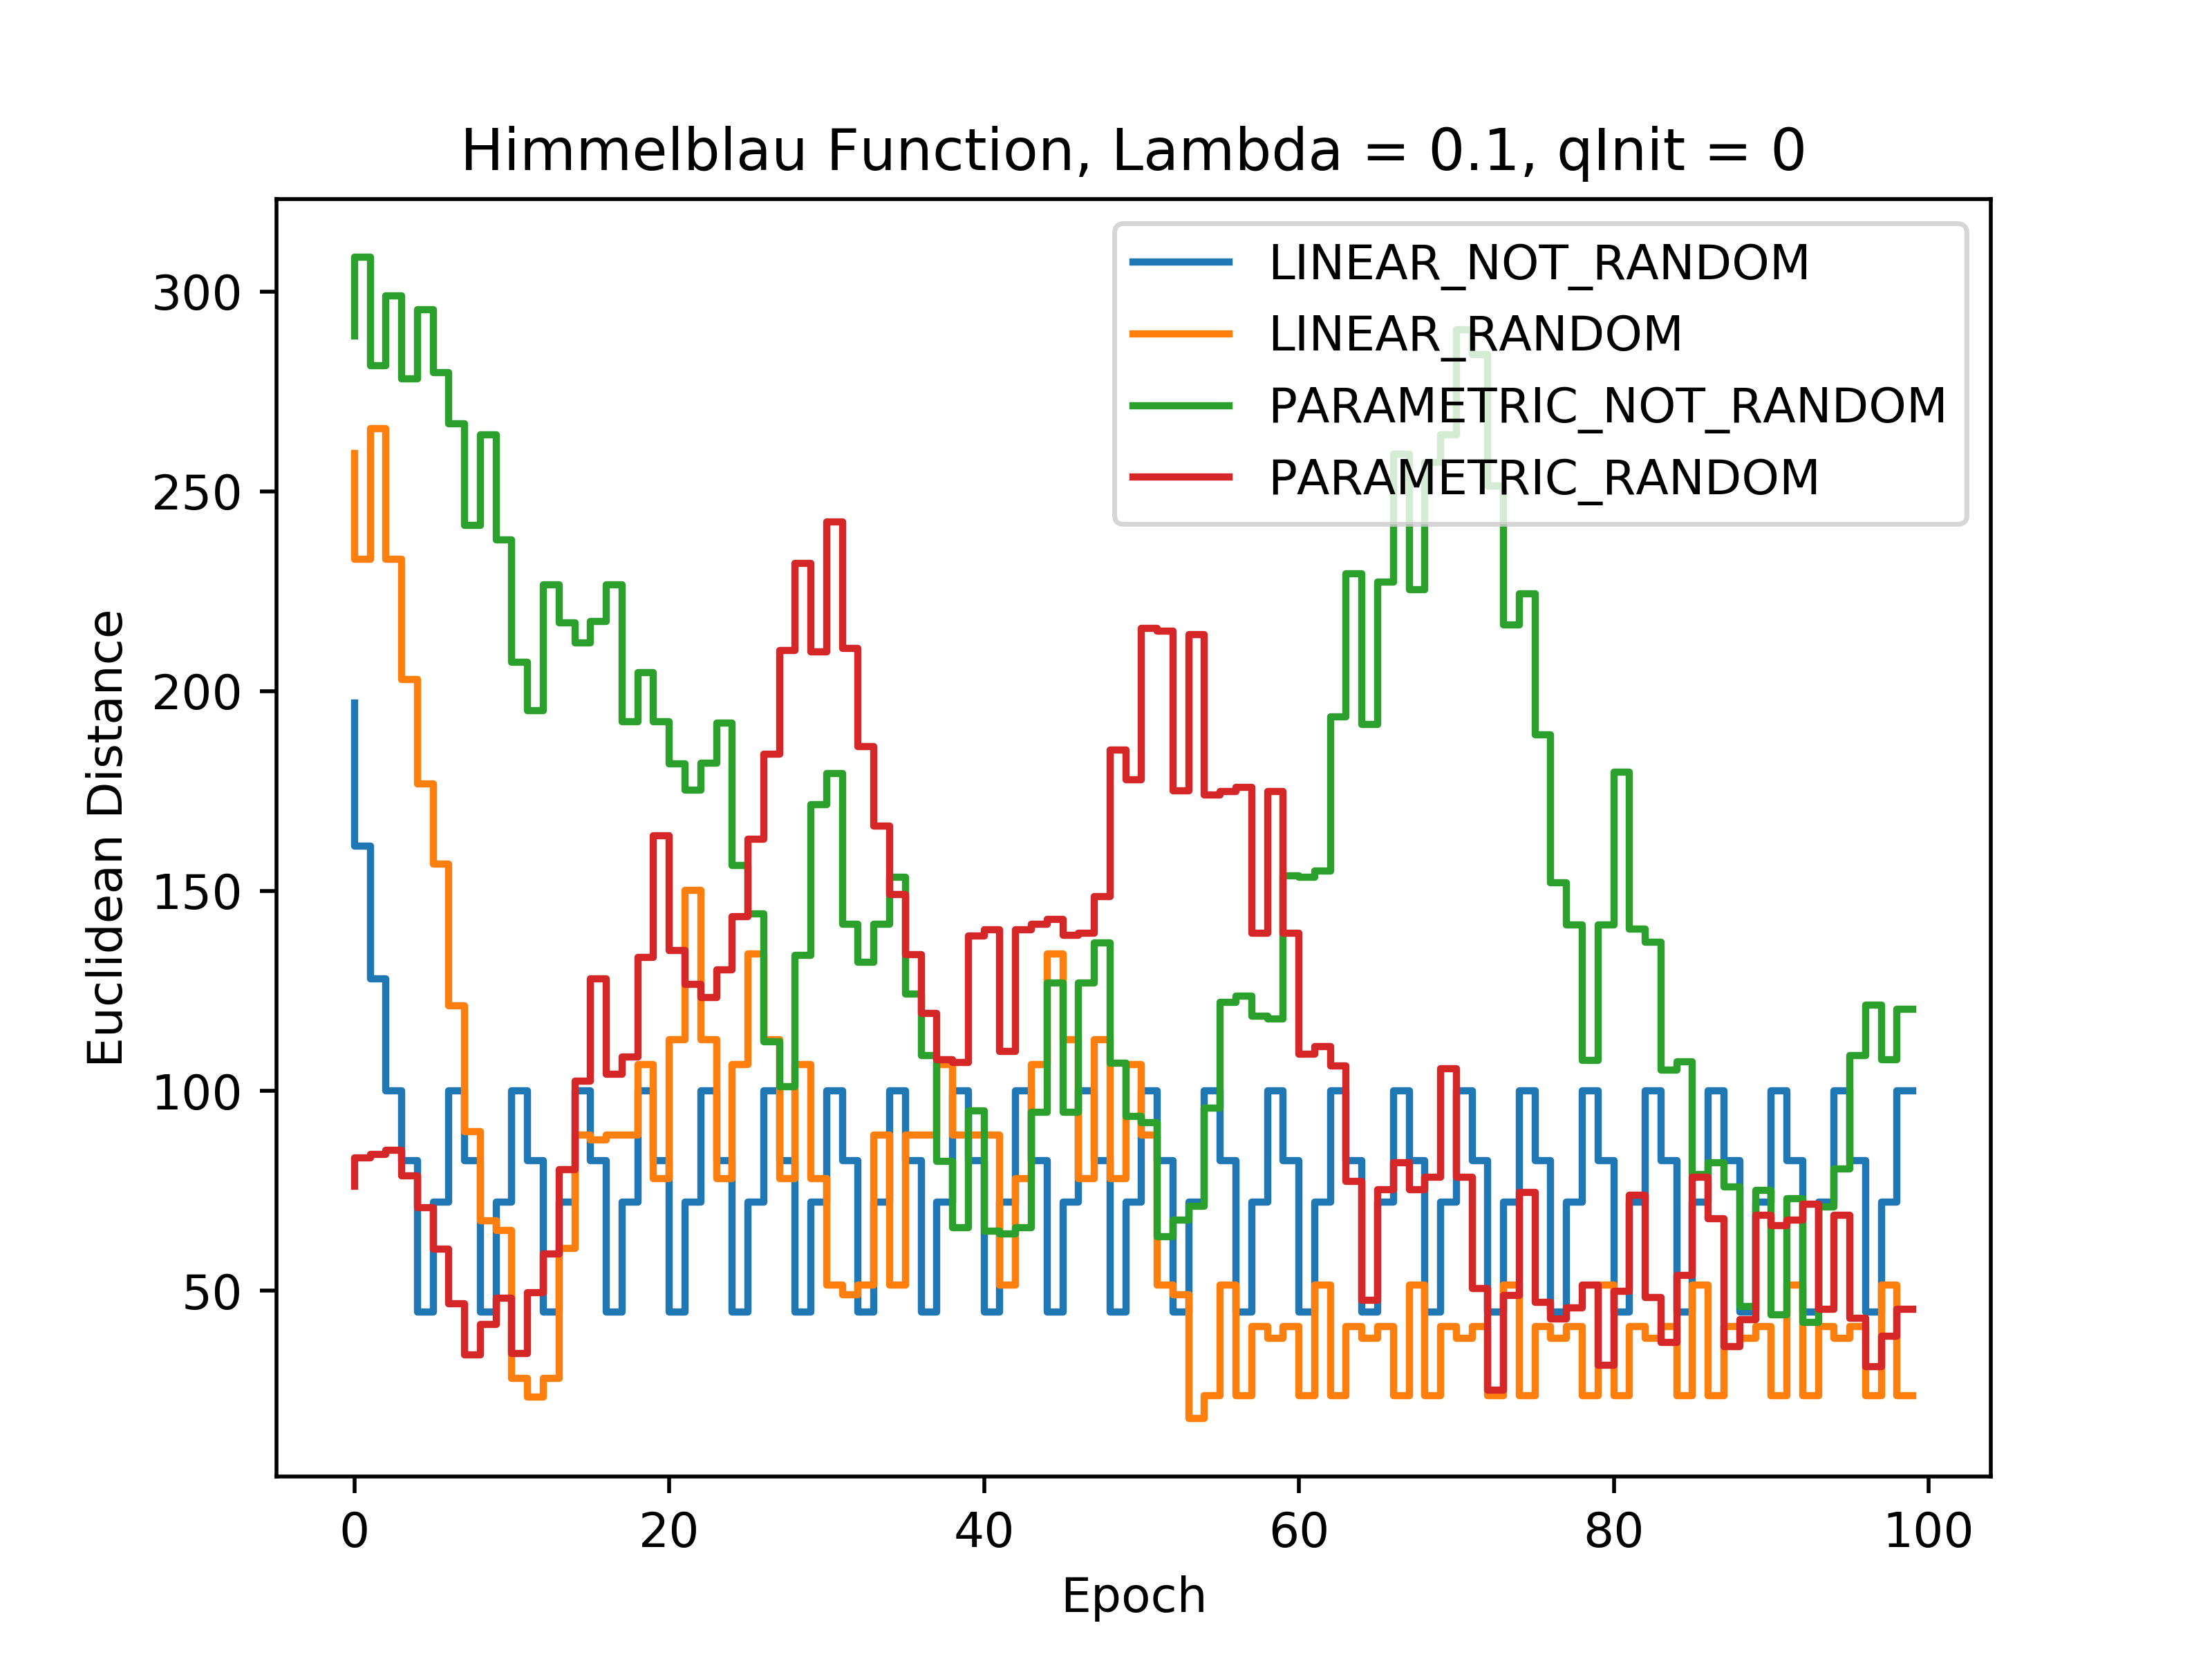
\includegraphics[width=0.4\textwidth]{HimmelblauDifference}
		}
		\subfigure[]{%
			\label{fig:HimmelblauValueFunction}
			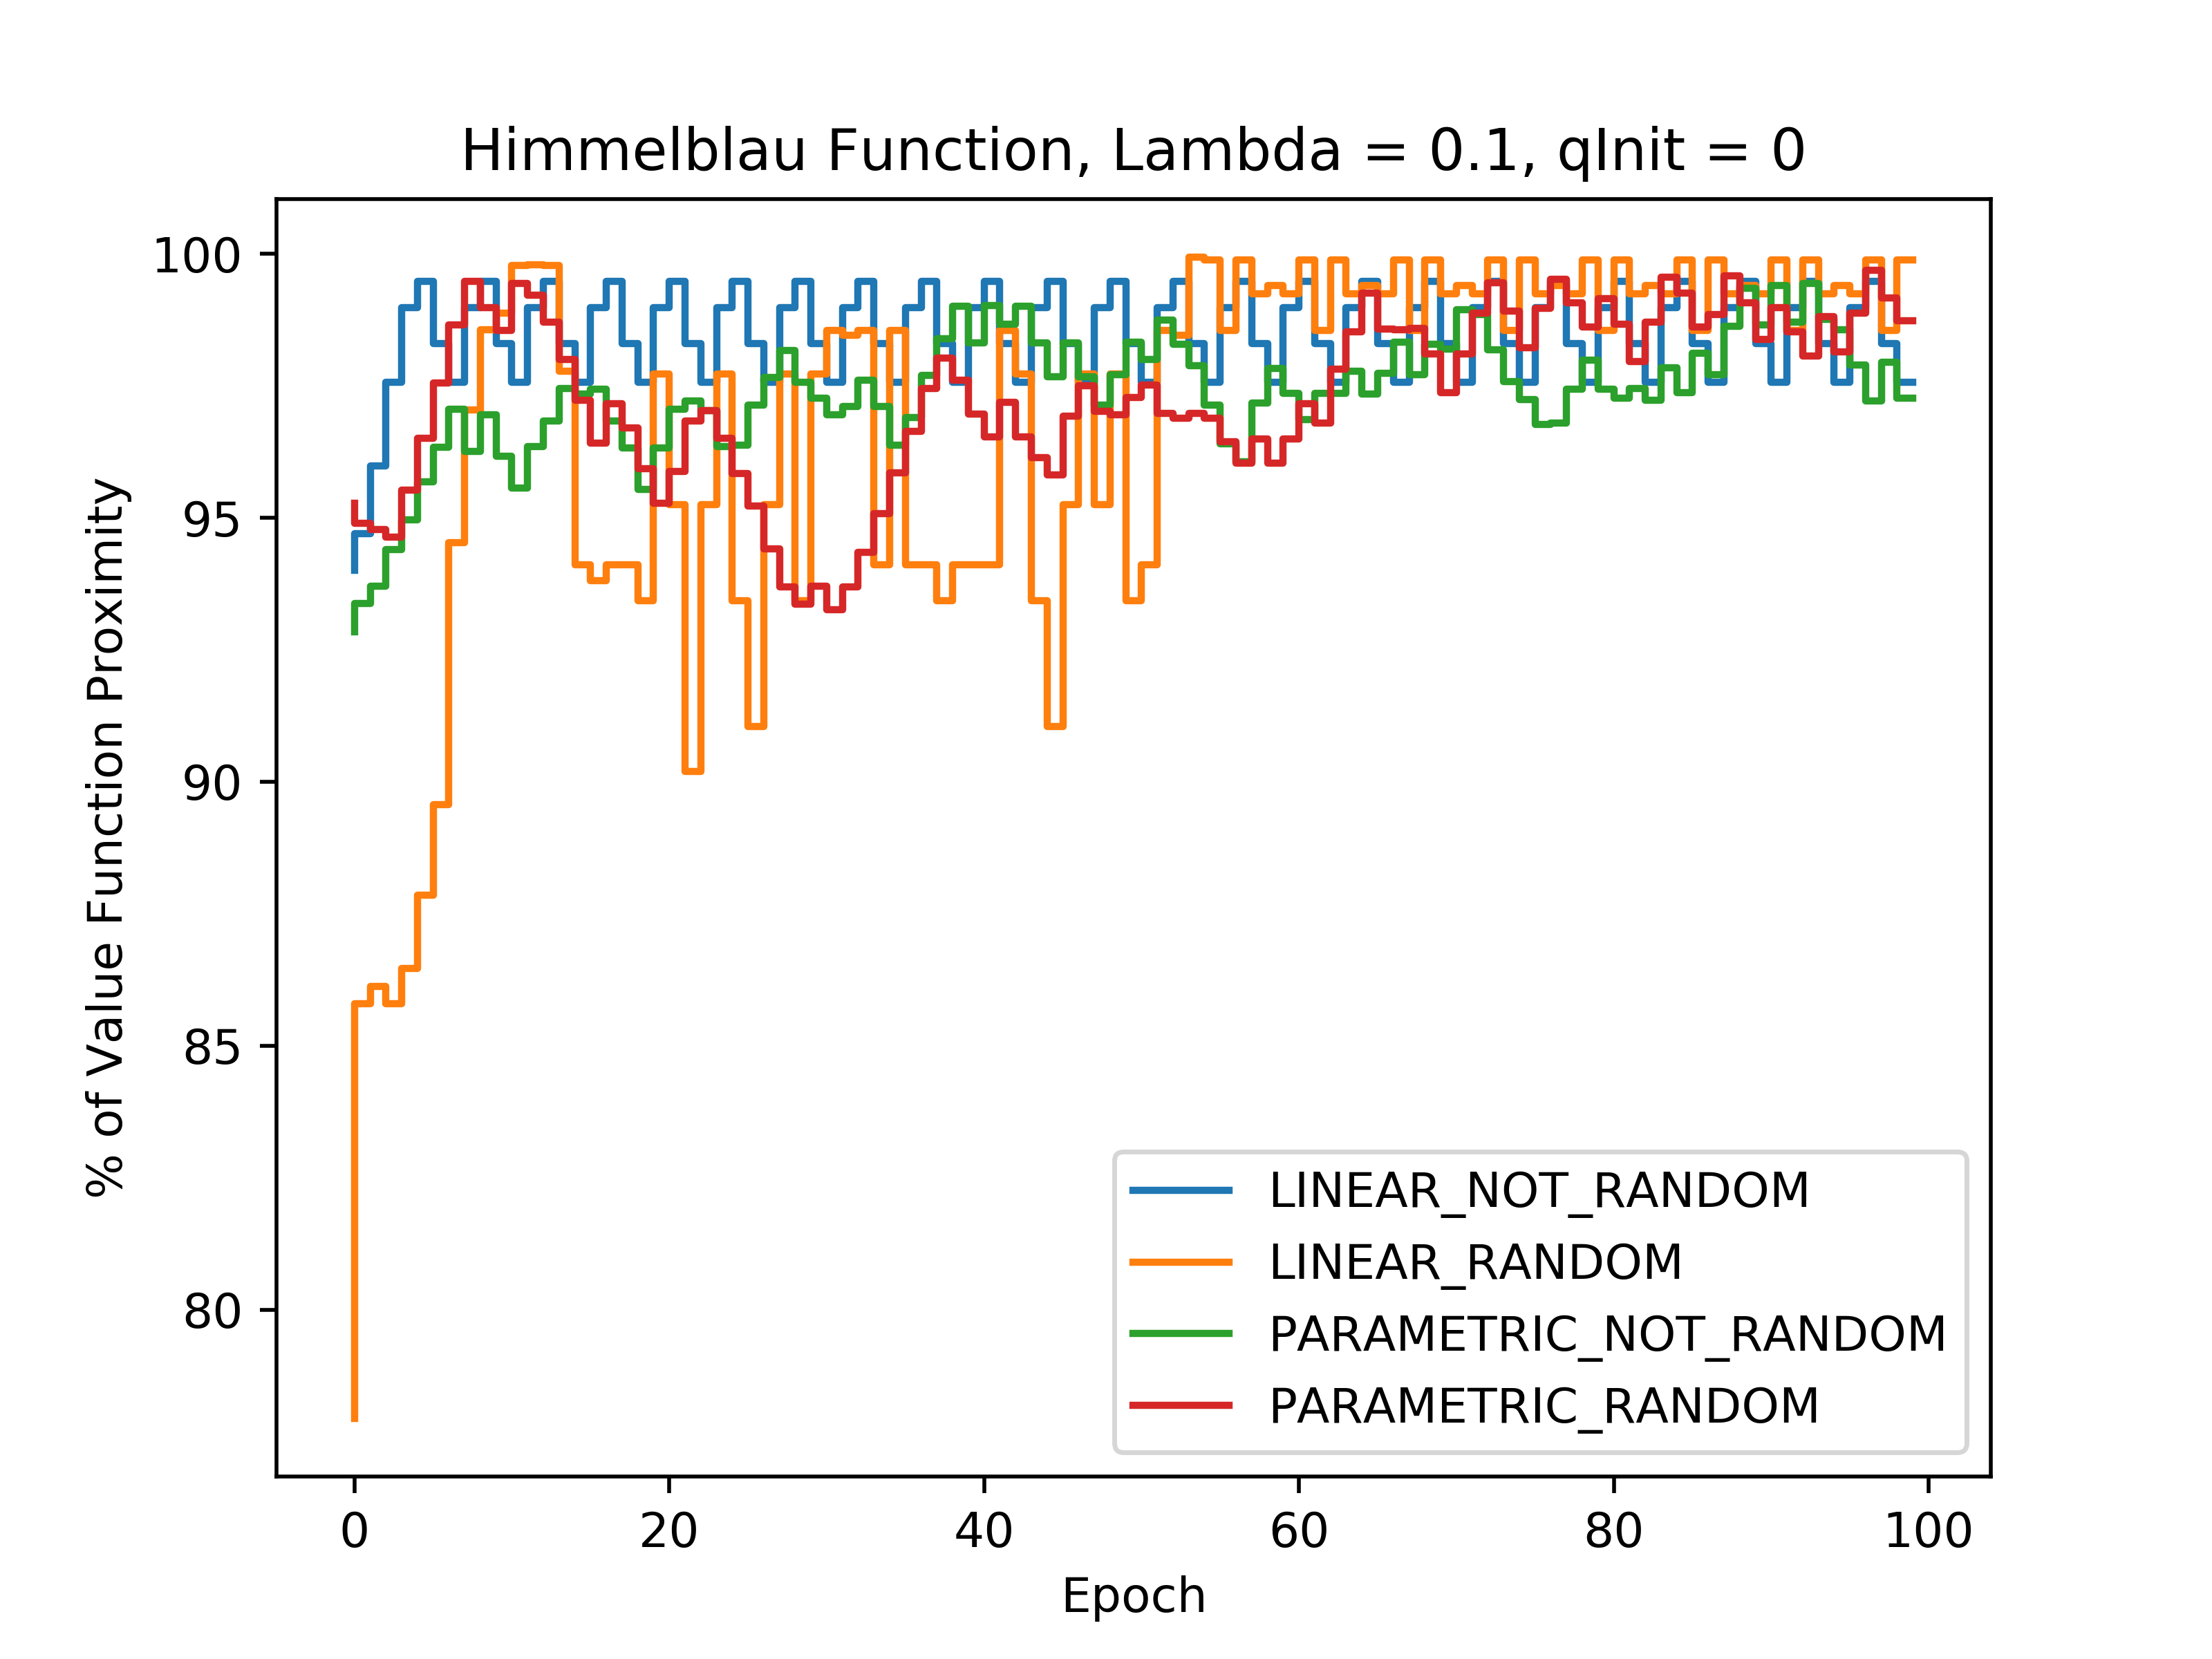
\includegraphics[width=0.4\textwidth]{HimmelblauValueFunction}
		}\\
		\subfigure[]{%
			\label{fig:HimmelblauGap}
			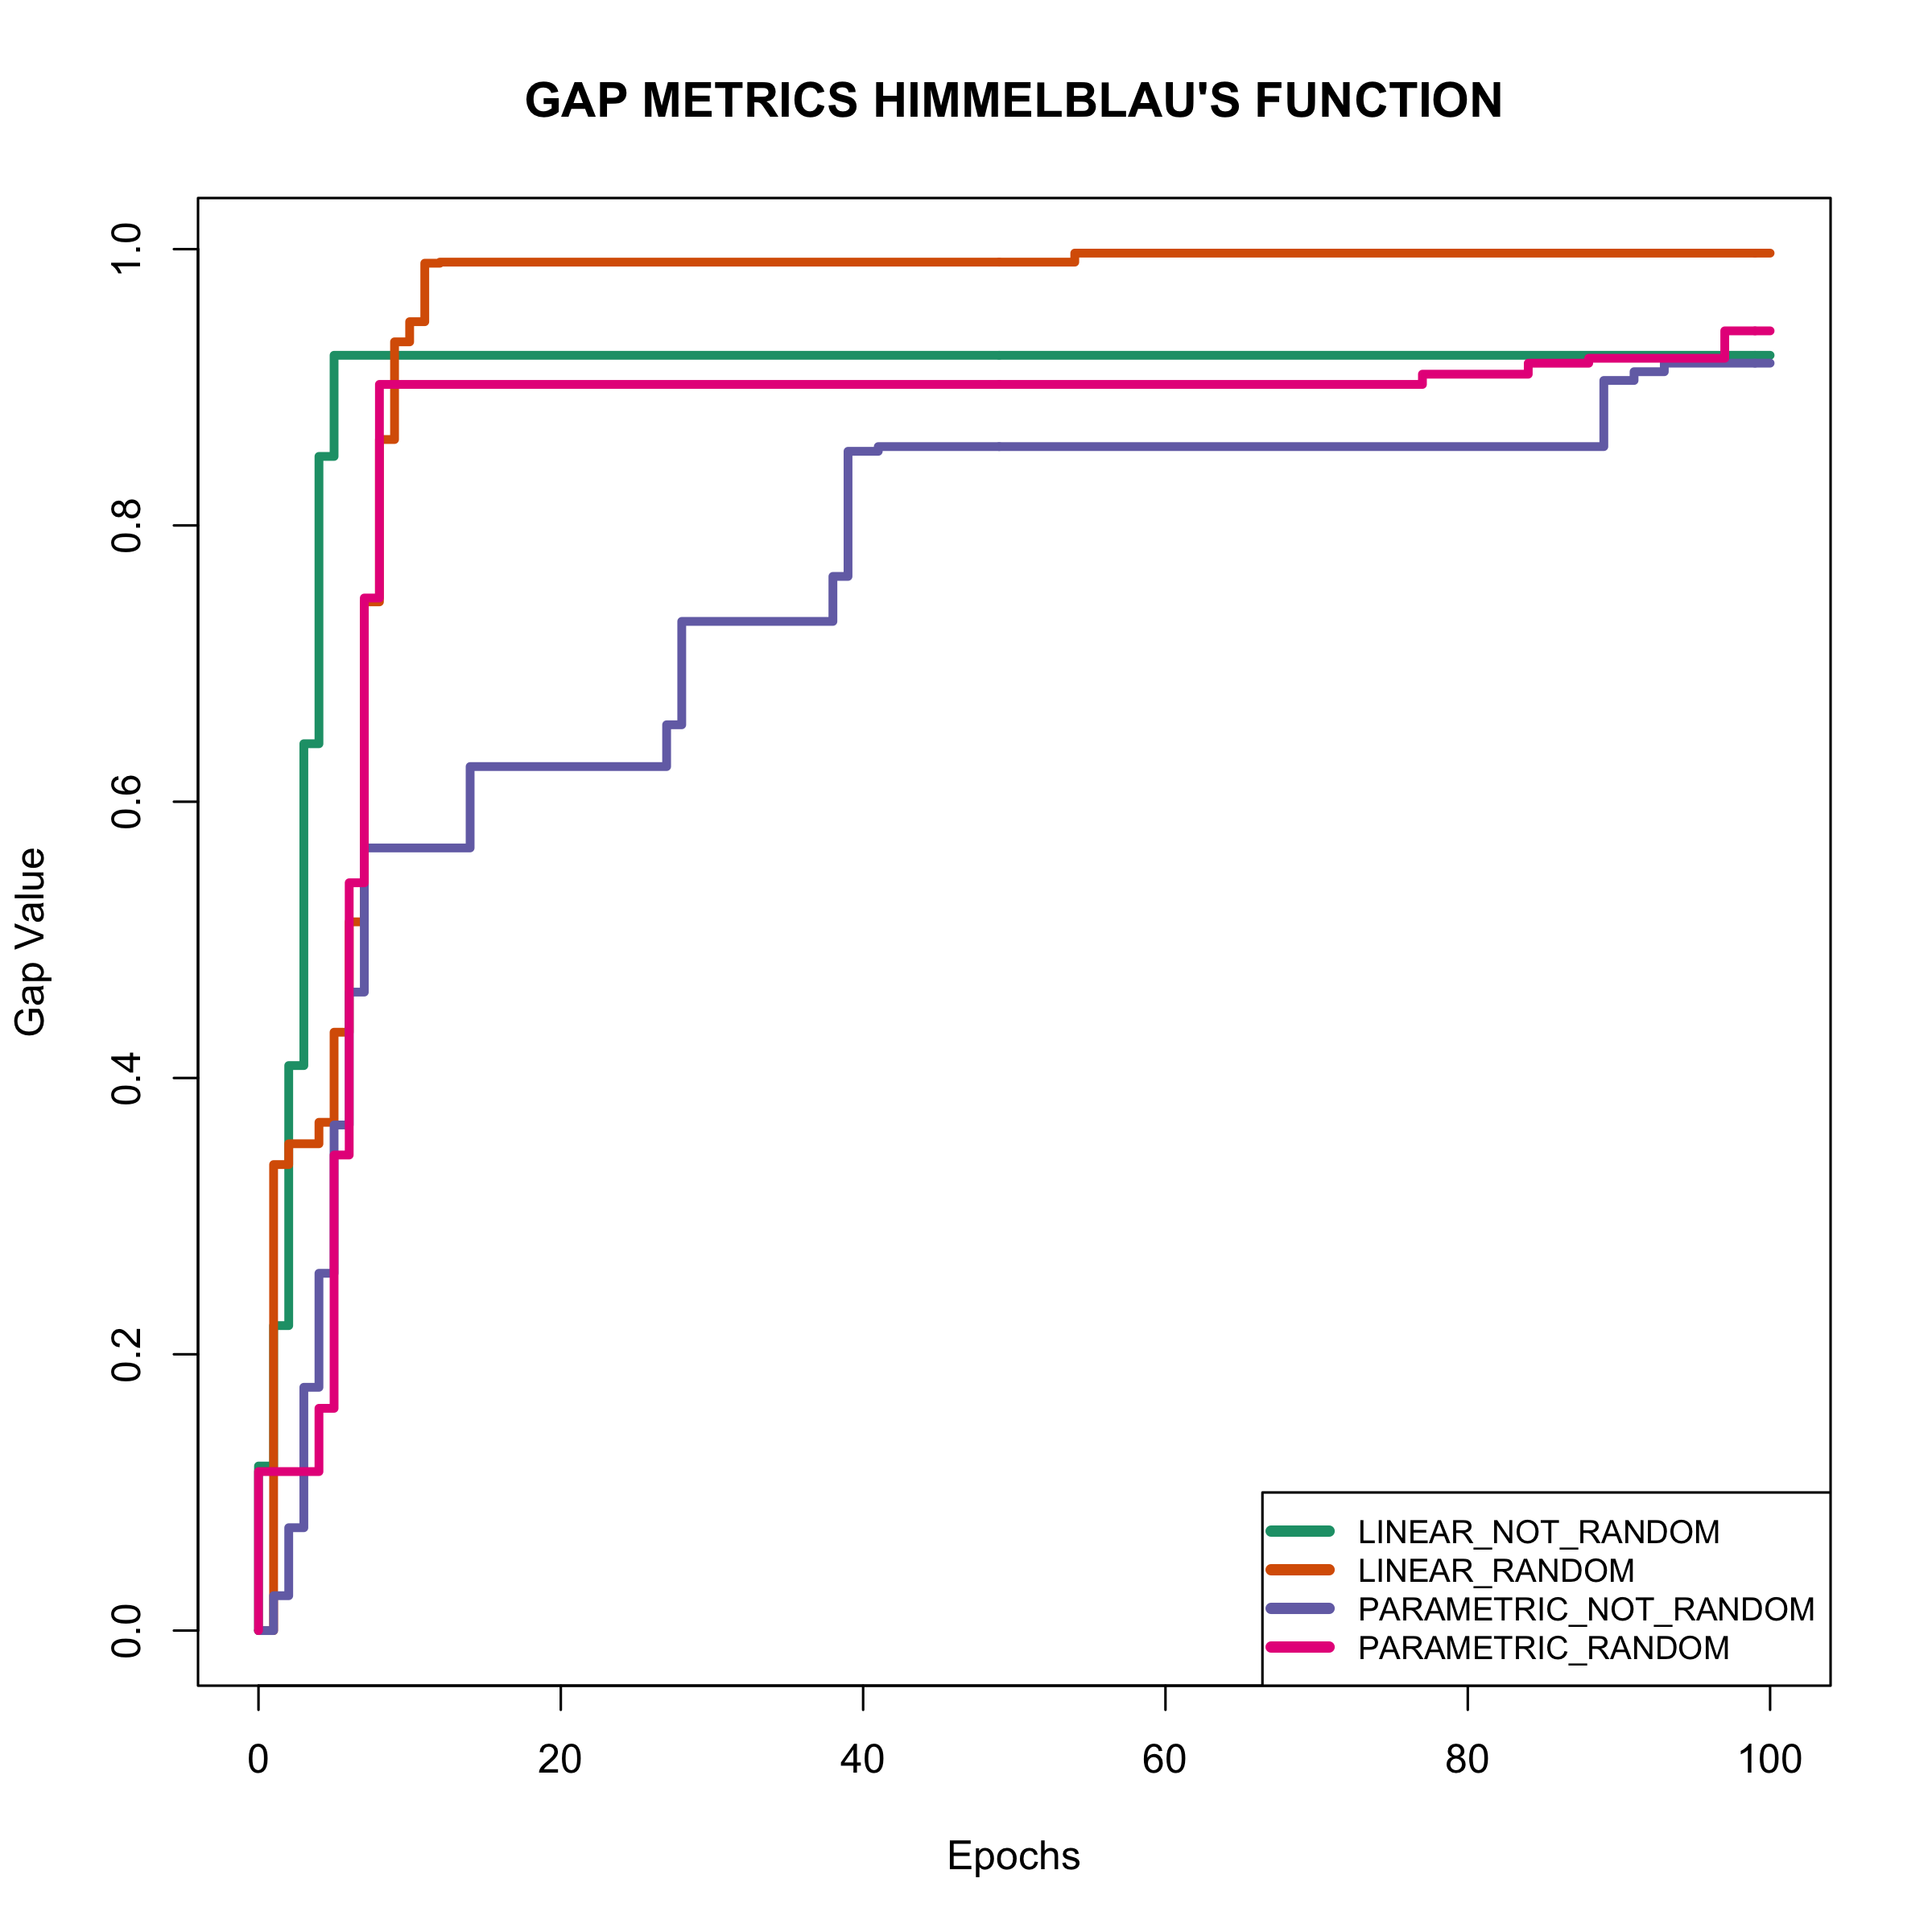
\includegraphics[width=0.4\textwidth]{HimmelblauGap}
		}		
	\end{center}
	\caption{
		Himmelblau' s Function.
	}
	\label{fig:HimmelblauResults}
\end{figure}

\subsection{Himmelblau' s Function} Plot (a) of figure \ref{fig:HimmelblauResults} graphically represents performances of the four possible declinations of {\tt SARSA($\lambda$)} algorithm obtained considering the \textit{Euclidean distance metric}. 

Looking at the {\tt linear, not random} declination's performance, it can be possible to note a starting high Euclidean difference between the agent's position and the global maximum. It decreases until epoch $5$. Starting from this epoch, a recurrent pattern starts to be developed. This behaviour depends on the fact that once the agent has achieved a good position compared to the maximum, it has to continue to make movements until the terminal state is achieved. Each movement implies a reward. The agent selects a set of movements that maximizes the reward and systematically repeats them. The stability just described is also proved by the fact that the standard deviation of the current declination is the lowest of the set with a value of $25.3$ (table $5.1$).

{\tt Linear, random} declination has a greater instability compared to the {\tt linear, not random} one. In the first fifty epochs the \textit{Euclidean distance} from the global maximum is constantly higher but then it starts to stabilize. Starting from the fiftieth epoch it develops a recurrent pattern and achieves best results. With an Euclidean distance mean of $71.6$ pixels from the maximum, it has the best performance of the set (table $5.1$).

The {\tt parametric, not random} declination has worst performances of the declinations' set. It is unable to minimize the Euclidean distance from the global maximum and it is highly unstable. Looking at table $5.1$ it is possible to note that the current declination as highest values in all statistic measures.

Finally, the {\tt parametric, random} declination selects a starting point near to the global maximum but it is unable to maintain a low Euclidean distance from it until epoch seventy. Starting from this epoch it develops a recurrent pattern similar to one previously described. Despite of this it is possible to say that its performances are worse compared to the first two ones.

Slower convergence of linear declinations compared to parametric ones depends on the fact that in the first case, as already explained in chapter $3$, greater movements are done at each epoch and a lower training time is required to achieve the maximum. The amount of parametric movements are strictly conditioned by the function's shape. If this represents an obstacle to a fast convergence, however it is an incentive to an higher precision. \\

\begin{table} [h!]
	\centering
	\resizebox{\linewidth}{!} {
	\begin{tabular}{c| cccccc}
		\hline \textbf{Himmelblau' s Function}
		& \textbf{Mean-ED} & \textbf{Standard deviation - ED}  \\ 
		\hline Linear not Random
		& $77.7$ &\cellcolor{red!25}$25.3$ \\ 
		\hline Linear Random
		& \cellcolor{red!25}$71.6$ & $52.2$ \\ 
		\hline Parametric not Random
		& $158.6$ & $71.3$ \\ 
		\hline Parametric Random
		& $105.5$ & $56.0$ \\ 
		\hline 
	\end{tabular}
}
\label{tab:HimmelblauTabEuclidean}
\caption{Euclidean Metric's Performances}
\end{table}

Plot (b) of figure ~\ref{fig:HimmelblauResults} graphically represents performances of the four possible declinations of {\tt SARSA($\lambda$)} algorithm obtained considering the \textit{Percentage of Value Function' s Proximity metric}.

All declinations, except for the {\tt linear, random} one, start with an high level of value function's proximity to the maximum. It depends on the function's shape. 

Once it has achieved a good enough proximal point to the maximum, the {\tt linear, not random} declination maintains always the same vale function's proximity level developing a recurrent pattern. The average level of proximity achieved by this declination is the best of the set (table $5.2$). The high stability of the current declination is proved by the lowest standard deviation of the set (table $5.2$). 

The {\tt linear, random} declination starts from a point not very close to the maximum in terms of value function's value. Its great instability reveals an inadequate training space. It starts to stabilize starting from the fiftieth epoch. Its starting instability is proved by the highest standard deviation of the set (table $5.2$).

The {\tt parametric, not random} declination reveals a general stability. The growth of proximity is slower then the corresponding linear declination because of the reduced amount of movement depending on the function's shape. 

Finally, the {\tt parametric, random} declination, as the corresponding linear declination, shows an initial instability. In general performances are more stable than the linear corresponding ones because of the lower amount of movement done at each epoch. Starting from the sixty-fifth epoch the proximity slowly grows and stabilizes. \\

\begin{table} [h!]
	\centering
	\resizebox{\linewidth}{!} {
	\begin{tabular}{c| cccccc} 
		\hline \textbf{Himmelblau' s Function}
		& \textbf{Mean- P} & \textbf{Standard deviation - P}  \\ 
		\hline Linear not Random
		& \cellcolor{green!25}$98.5$ & \cellcolor{green!25}$0.96$  \\ 
		\hline Linear Random
		& $96.8$ & $4.0$ \\ 
		\hline Parametric not Random
		& $97.4$ & $1.2$ \\ 
		\hline Parametric Random
		& $97.3$ & $1.6$ \\ 
		\hline 
	\end{tabular}
}
\label{HimmelblauTabProximity}
\caption{Value Function' s Proximity.} 
\end{table}

Plot (c) of figure ~\ref{fig:HimmelblauResults} graphically represents performances of the four possible declinations of {\tt SARSA($\lambda$)} algorithm obtained considering the \textit{gap metric}. According to this plot the most effective declination of {\tt SARSA($\lambda$)} algorithm in finding the maximum is the {\tt linear, random} one. Looking at table $5.9$ it is possible to note that {\tt linear, random} declination achieves point $(3.67, -1.57)$ with a value function of $2498.457$ out of $2500.0$.

\begin{figure}[h!]
	\begin{center}
		\subfigure[]{%
			\label{fig:ParabolicDifference}
			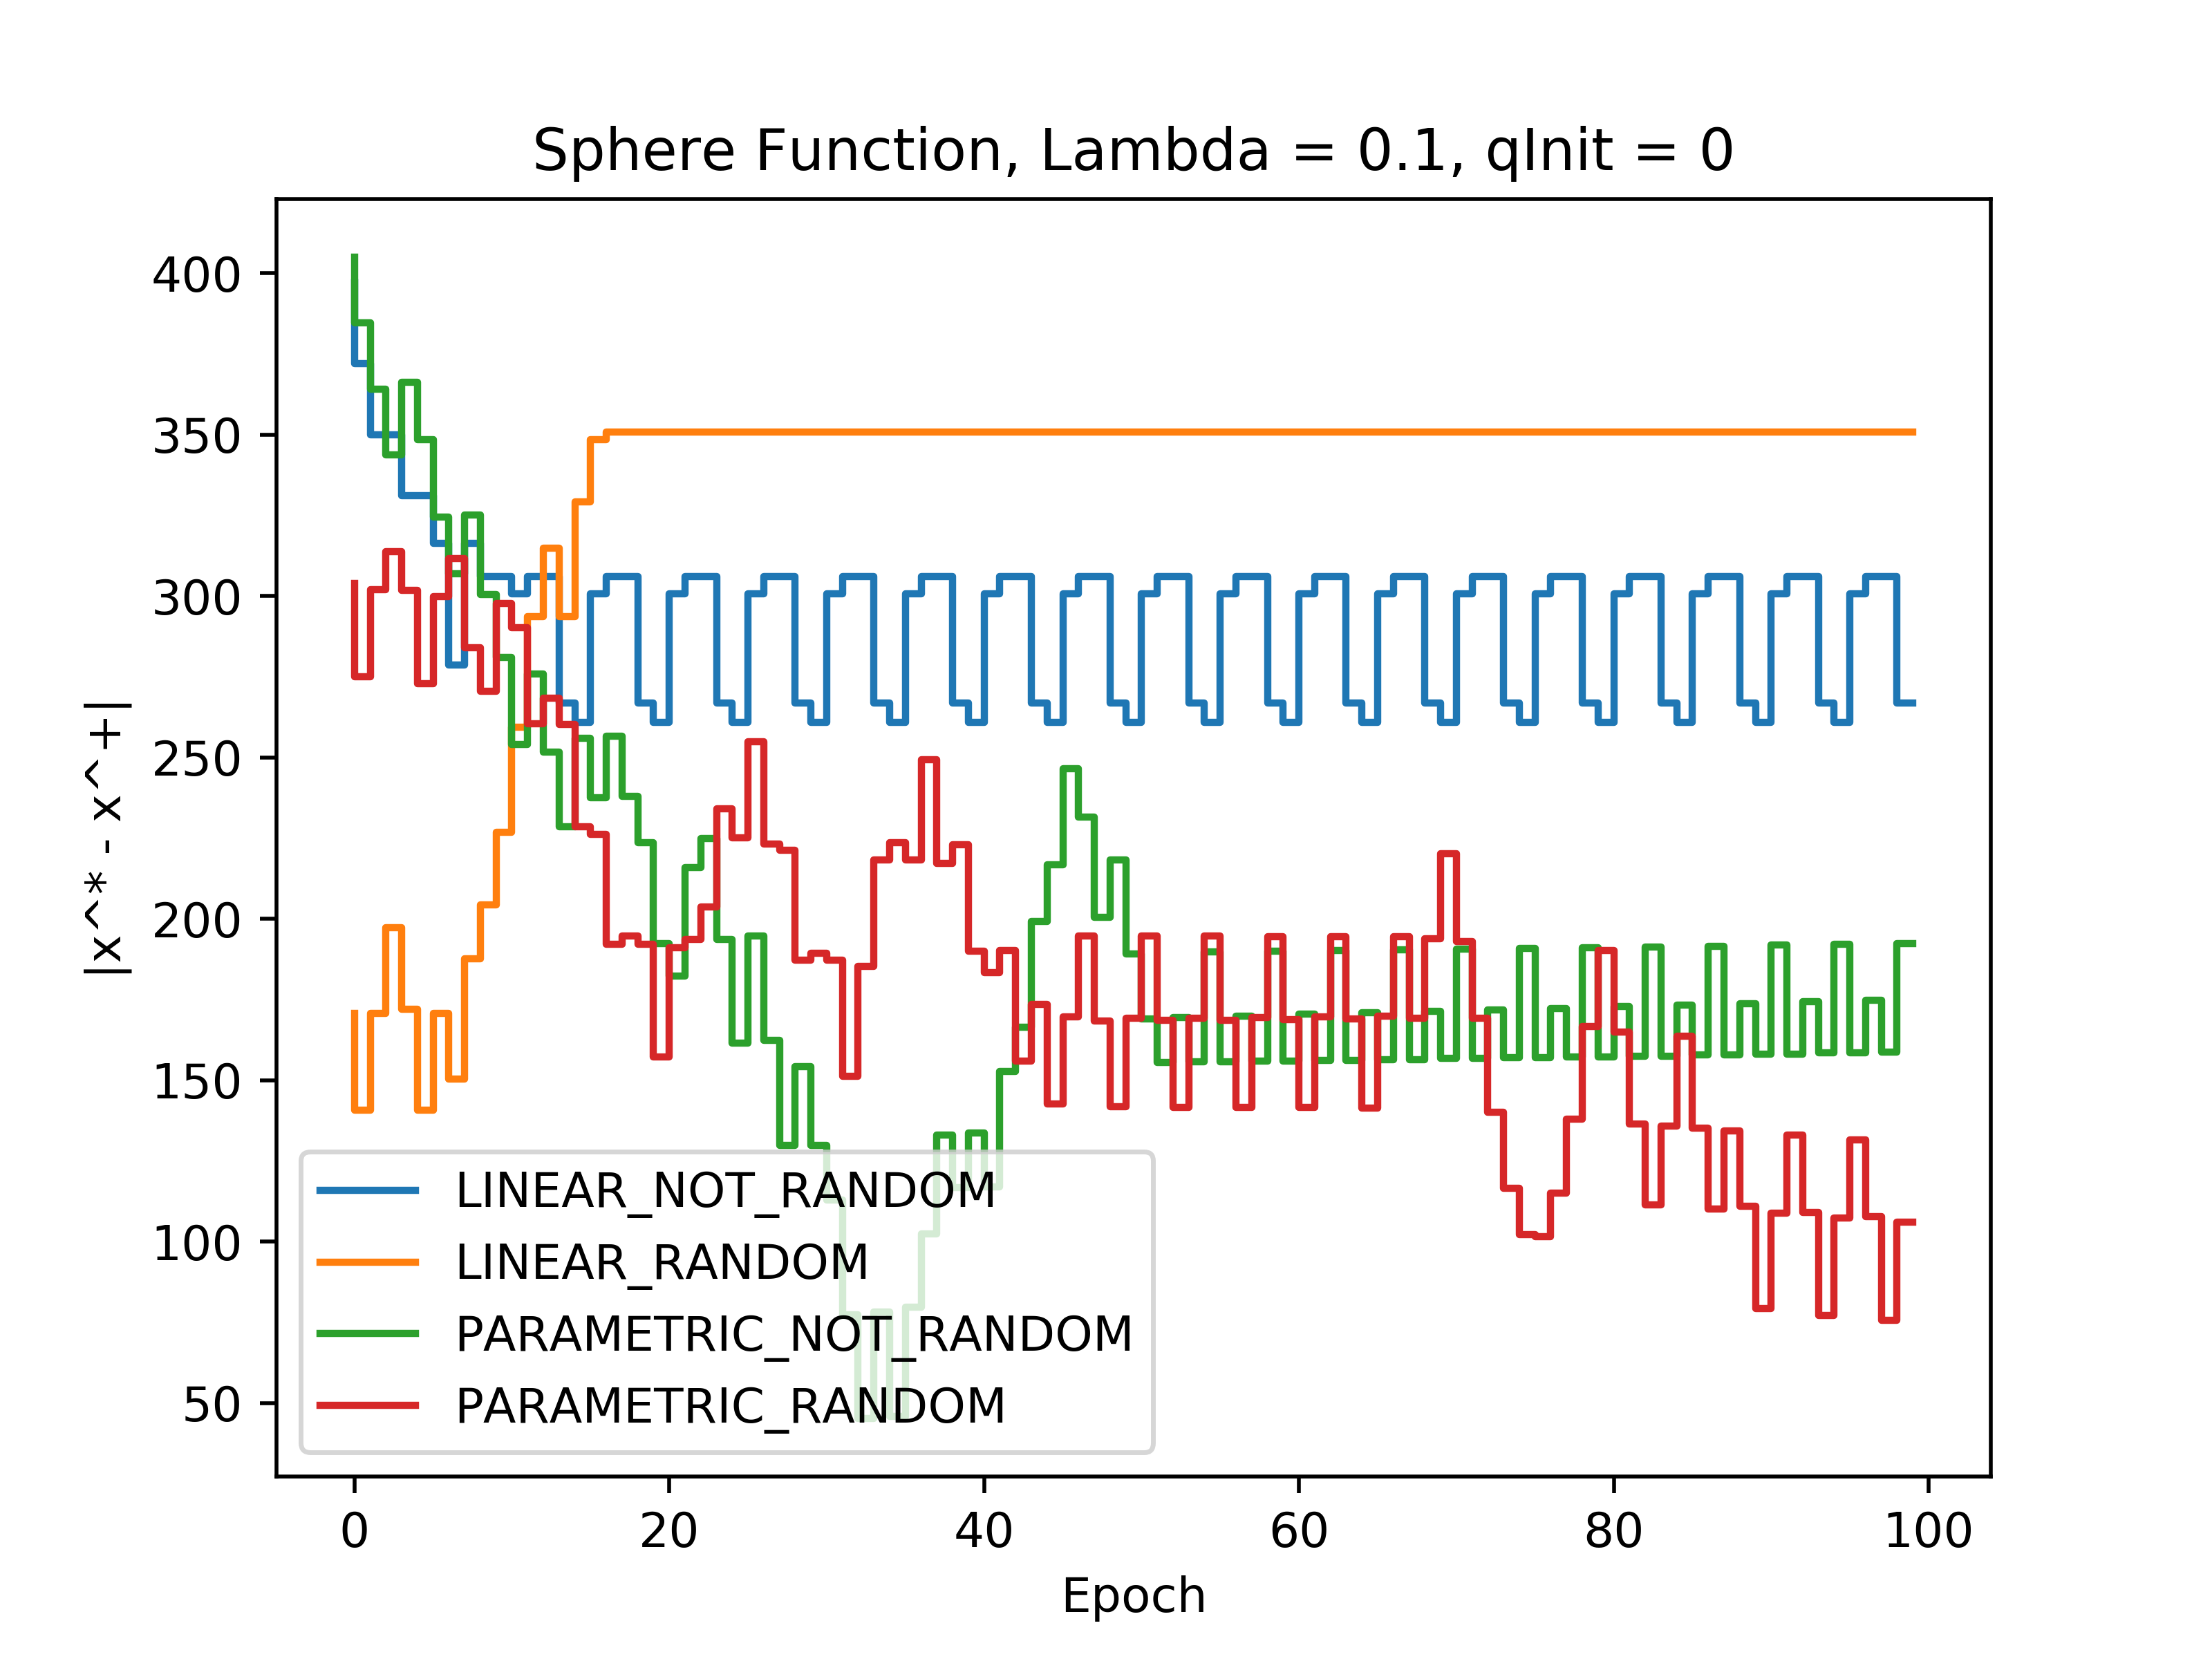
\includegraphics[width=0.4\textwidth]{ParabolicEuclidean}
		}
		\subfigure[]{%
			\label{fig:ParabolicValueFunction}
			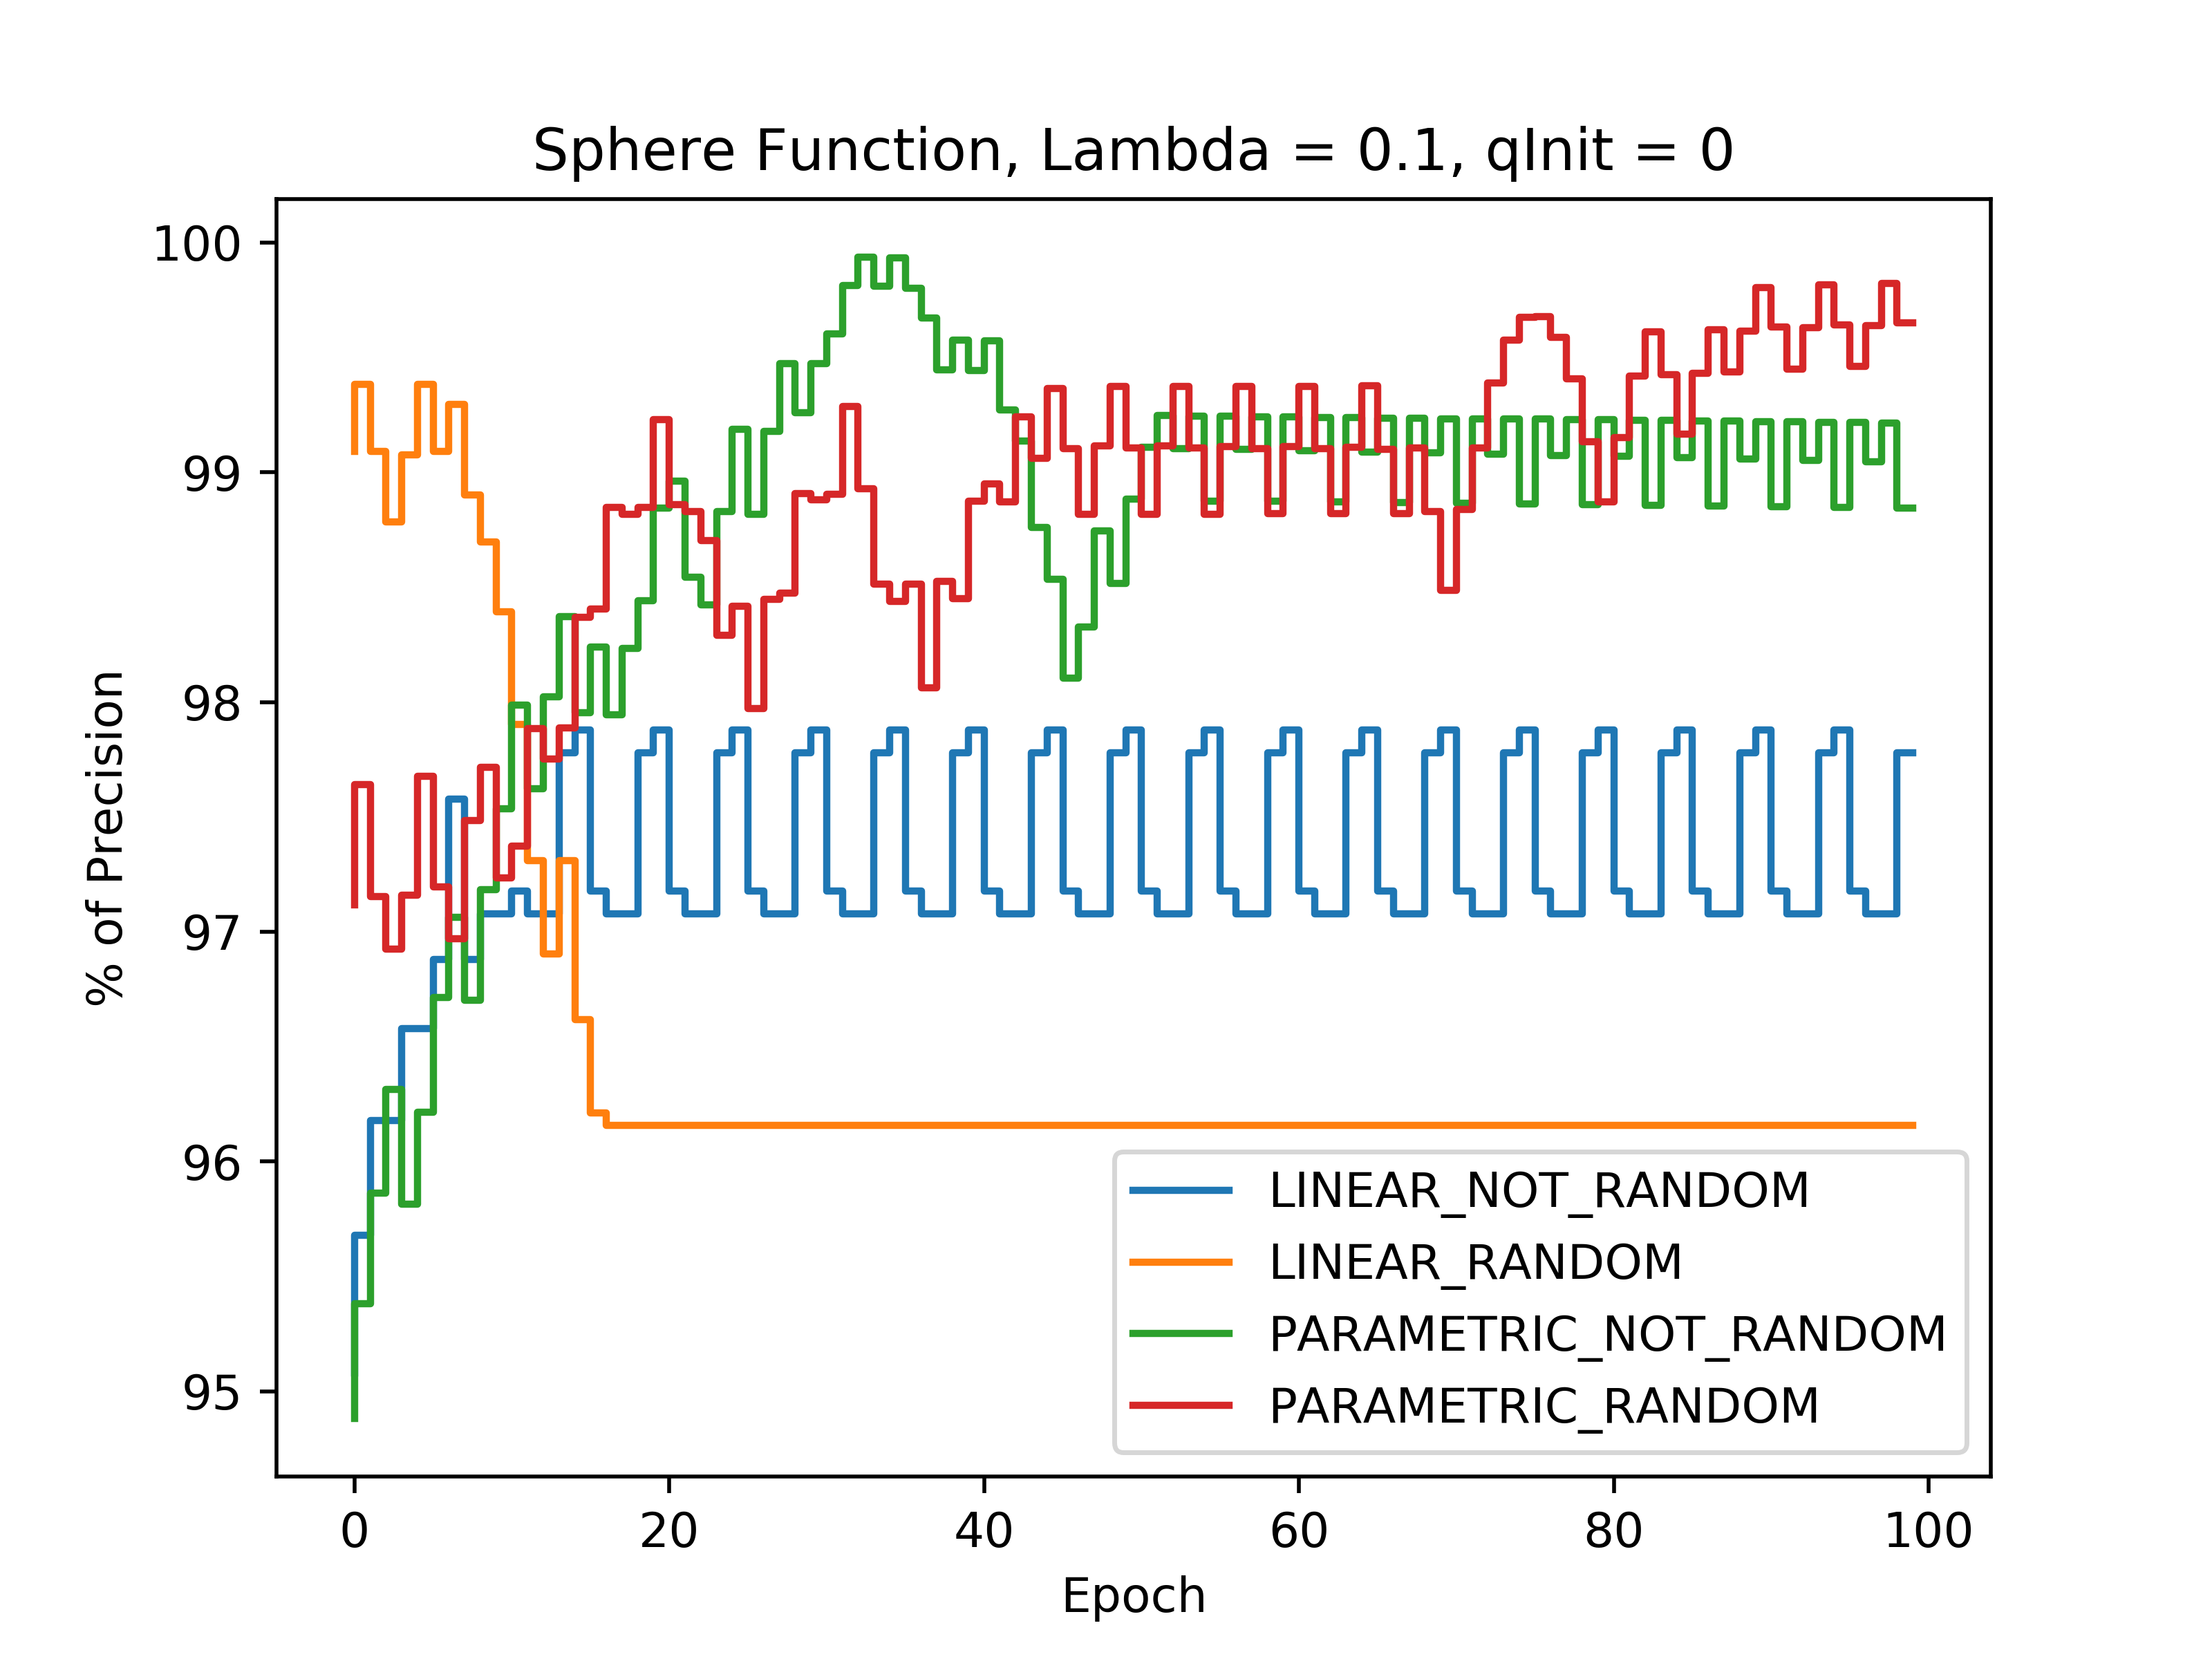
\includegraphics[width=0.4\textwidth]{SphereValueFunction}
		}\\
		\subfigure[]{%
			\label{fig:ParabolicGap}
			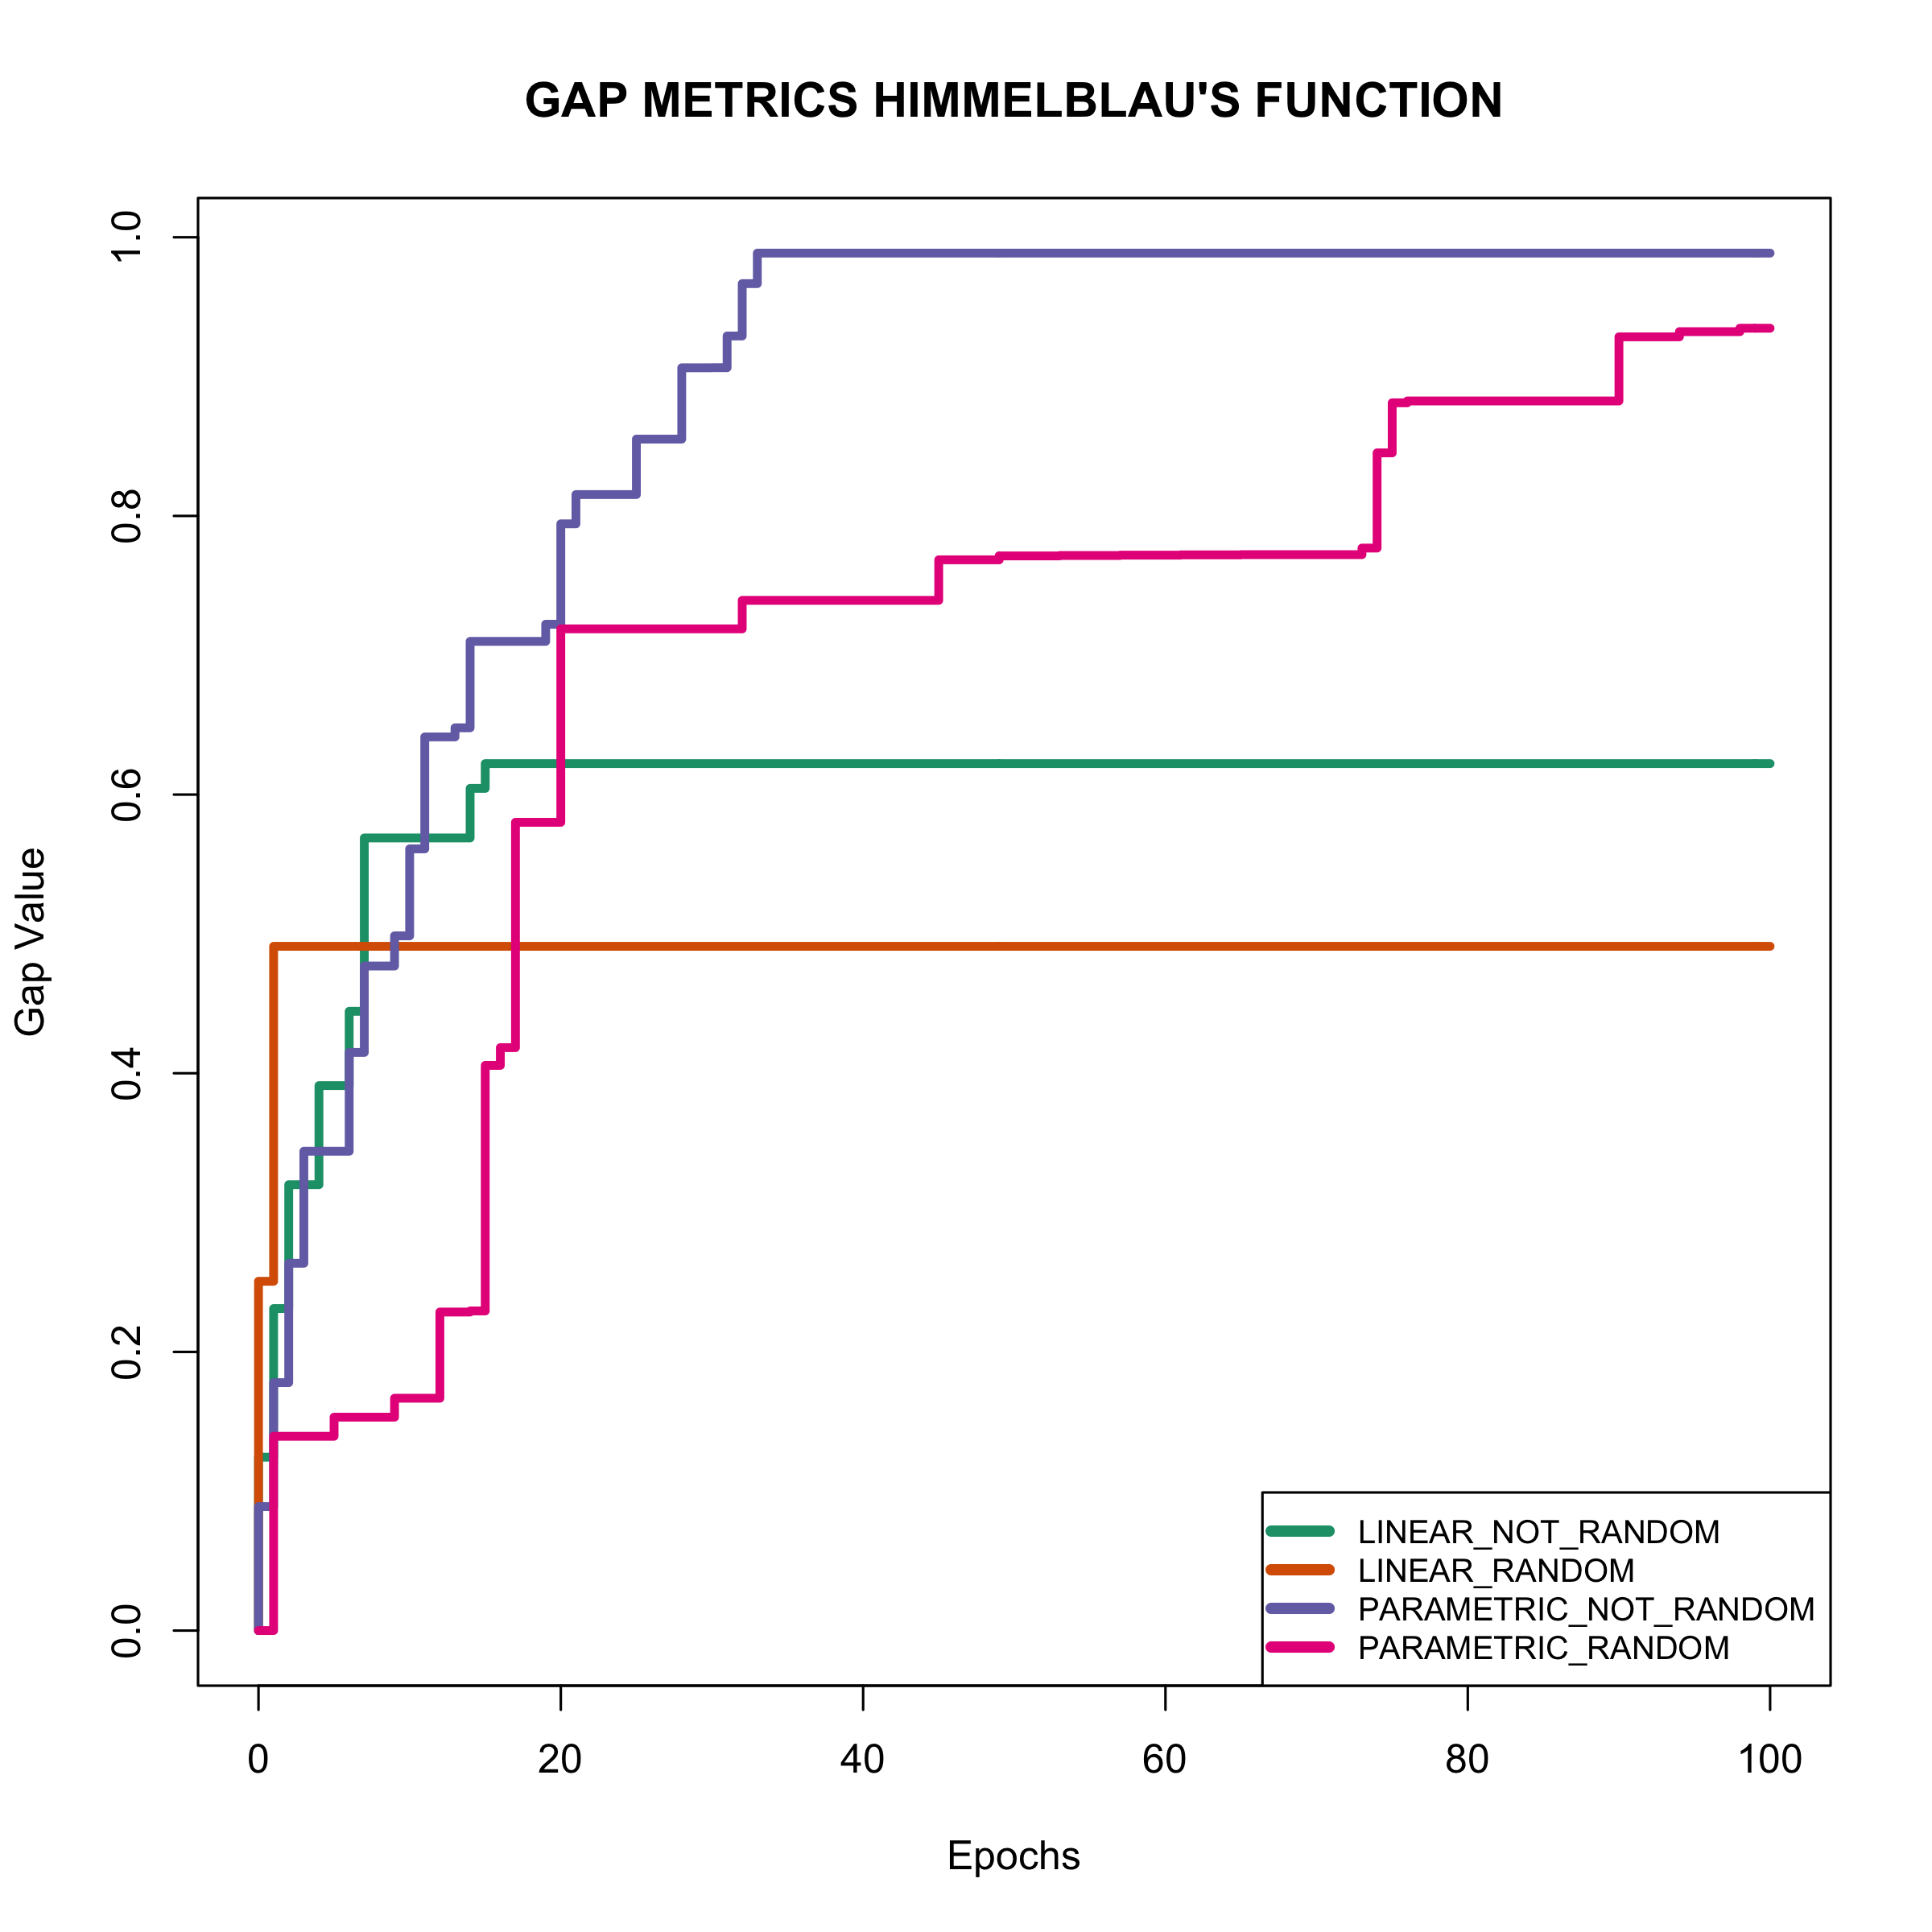
\includegraphics[width=0.4\textwidth]{ParabolicGap}
		} \\
		
	\end{center}
	\caption{
		Sphere Function.
	}
	\label{fig:ParabolicResults}
\end{figure}


\subsection{Sphere Function} Before starting to analyse performances of different declinations of {\tt SARSA($\lambda$)} algorithm in maximizing the Sphere function, it is important to underline that the starting point for the current function in non-random declinations is $(0, 0)$. The reason for this choice is that $f(300, 300)$ is itself the maximum of the function. \\

Plot (a) of figure ~\ref{fig:ParabolicResults} graphically represents performances of the four possible declinations of {\tt SARSA($\lambda$)} algorithm obtained considering the \textit{Euclidean distance metric}. Looking at the {\tt linear, not random} declination it is possible to note a constant, high Euclidean difference between the agent's position and the global maximum. This distance never decreases and still from the first epochs, a recurrent pattern starts to be developed. The inefficiency of the algorithm's declination depends on an inadequate training space. The relationship between different explored states and total possible states does not permit the agent to develop an efficient policy. Bad performance's results of the current declination are also certified by an high metric's average (table $5.3$). On the other hand the great stability of this declination is underlined by the lowest standard deviation of the set (table $5.3$).

{\tt Linear, random} declination starts from a point relatively close to the maximum, but, one more time, the inadequate training space prevents its to develop a rally optimal policy. This declination is the less efficient one with an average Euclidean distance from the maximum of $328.9$ pixels.

Better performances can be registered looking at parametric declinations of the algorithm. The {\tt parametric, not random} declination starts with a physiological high Euclidean difference from the maximum. It rapidly decreases until the thirty-fifth epoch and then it has another soft increase. Starting from the fifty-fifth epoch a recurrent pattern starts to be developed. Despite of the fact that this declination is the most unstable one with a standard deviation of $67.9$ (table $5.3$), it has one of the lowest average Euclidean distance from the maximum. 

The {\tt parametric, random} declination of {\tt SARSA($\lambda$)} algorithm has the best performance of the set. After a starting, considerable instability it reaches an Euclidean difference of around fifty pixels. The good performance is also proved by the fact that the average Euclidean distance from the maximum is $185.3$ pixels. \\

\begin{table}[h!]
	\centering
	\resizebox{\linewidth}{!} {
	\begin{tabular}{c| cccccc} 
		\hline \textbf{Sphere Function}
		& \textbf{Mean-ED} & \textbf{Standard deviation - ED} \\ 
		\hline Linear not Random
		& $293.2$ &\cellcolor{red!25} $25.6$  \\ 
		\hline Linear Random
		& $328.9$ & $56.3$ \\ 
		\hline Parametric not Random
		& $190.7$ & $67.9$ \\ 
		\hline Parametric Random
		& \cellcolor{red!25} $185.3$ & $58.0$ \\ 
		\hline 
	\end{tabular} 
}
\label{ParabolicTabEuclidean}
\caption{Euclidean Metric's Performances}
\end{table}

Plot (b) of figure ~\ref{fig:ParabolicResults} graphically represents performances of the four possible declinations of {\tt SARSA($\lambda$)} algorithm obtained considering the \textit{Percentage of Value Function' s Proximity metric}. 

The {\tt linear, not random} declination starts from a value function's proximity of about $97.5\%$ from the maximum. It is completely unable to improve this percentage. Already starting from the first epochs it develops a recurrent pattern. This behaviour allows its to have the lowest standard deviation of the declinations' set (table $5.4$). Unfortunately the value function's proximity mean is the second lowest one. 
 
The {\tt linear, random} declination starts from a very high value function's proximity level. Because of an inadequate training space it decreases until the twentieth epoch. Starting from this epoch it stars to stabilize. Effects of this behaviour on the average value function's proximity to the maximum and on average standard deviation are relevant.
 
The {\tt parametric, not random} declination is the most unstable one. It starts with a low value function's proximity level and slowly grows achieving peaks of about $100\%$. Starting from the fiftieth epoch it stabilizes developing a recurrent pattern. The initial high instability has effects on average value function's proximity variance making its the highest one (table $5.4$).
 
The {\tt parametric, random} declination of {\tt SARSA($\lambda$)} algorithm is the most efficient one. It starts with a value function's proximity level of about $97\%$ and slowly grows first stabilizing around $99\%$ and than growing more achieving peaks of $99.8\%$. Looking at table $5.4$ it is possible to note that the average value function's proximity is the highest one with a level of $98.8\%$.
 
In this case it is possible to underline that parametric declinations do better than linear ones. In particular the random starting position allows the agent to develop a better policy. The main reason of the failure of non random declinations is the reduced training space compared to the distance between the starting point and the maximum.

\begin{table}[h!]
	\centering
	\resizebox{\linewidth}{!} {
	\begin{tabular}{c| cccccc} 
		\hline \textbf{Sphere Function}
		& \textbf{Mean- P} & \textbf{Standard deviation - P} \\ 
		\hline Linear not Random
		& $97.3$ & \cellcolor{green!25}$0.49$ \\ 
		\hline Linear Random
		& $95.5$ & $0.92$ \\ 
		\hline Parametric not Random
		& $98.7$ & $0.98$ \\ 
		\hline Parametric Random
		& \cellcolor{green!25}$98.8$ & $0.72$ \\ 
		\hline 
	\end{tabular} 
}
\label{ParabolicTabProximity}
\caption{Value Function' s Proximity.} 
\end{table}

Plot (c) of figure ~\ref{fig:HimmelblauResults} graphically represents performances of the four possible declinations of {\tt SARSA($\lambda$)} algorithm obtained using the \textit{gap metric}. According to this plot the most effective declination of {\tt SARSA($\lambda$)} algorithm in finding the maximum is the {\tt parametric, not random} one. Looking at table $5.9$ it is possible to note that {\tt parametric, not random} declination achieves point $(-1.033, -1.099)$ with a value function of $3557.722$ out of $3560.0$.

\begin{figure}[h!]
	\begin{center}
		\subfigure[]{%
			\label{fig:BealeDifference}
			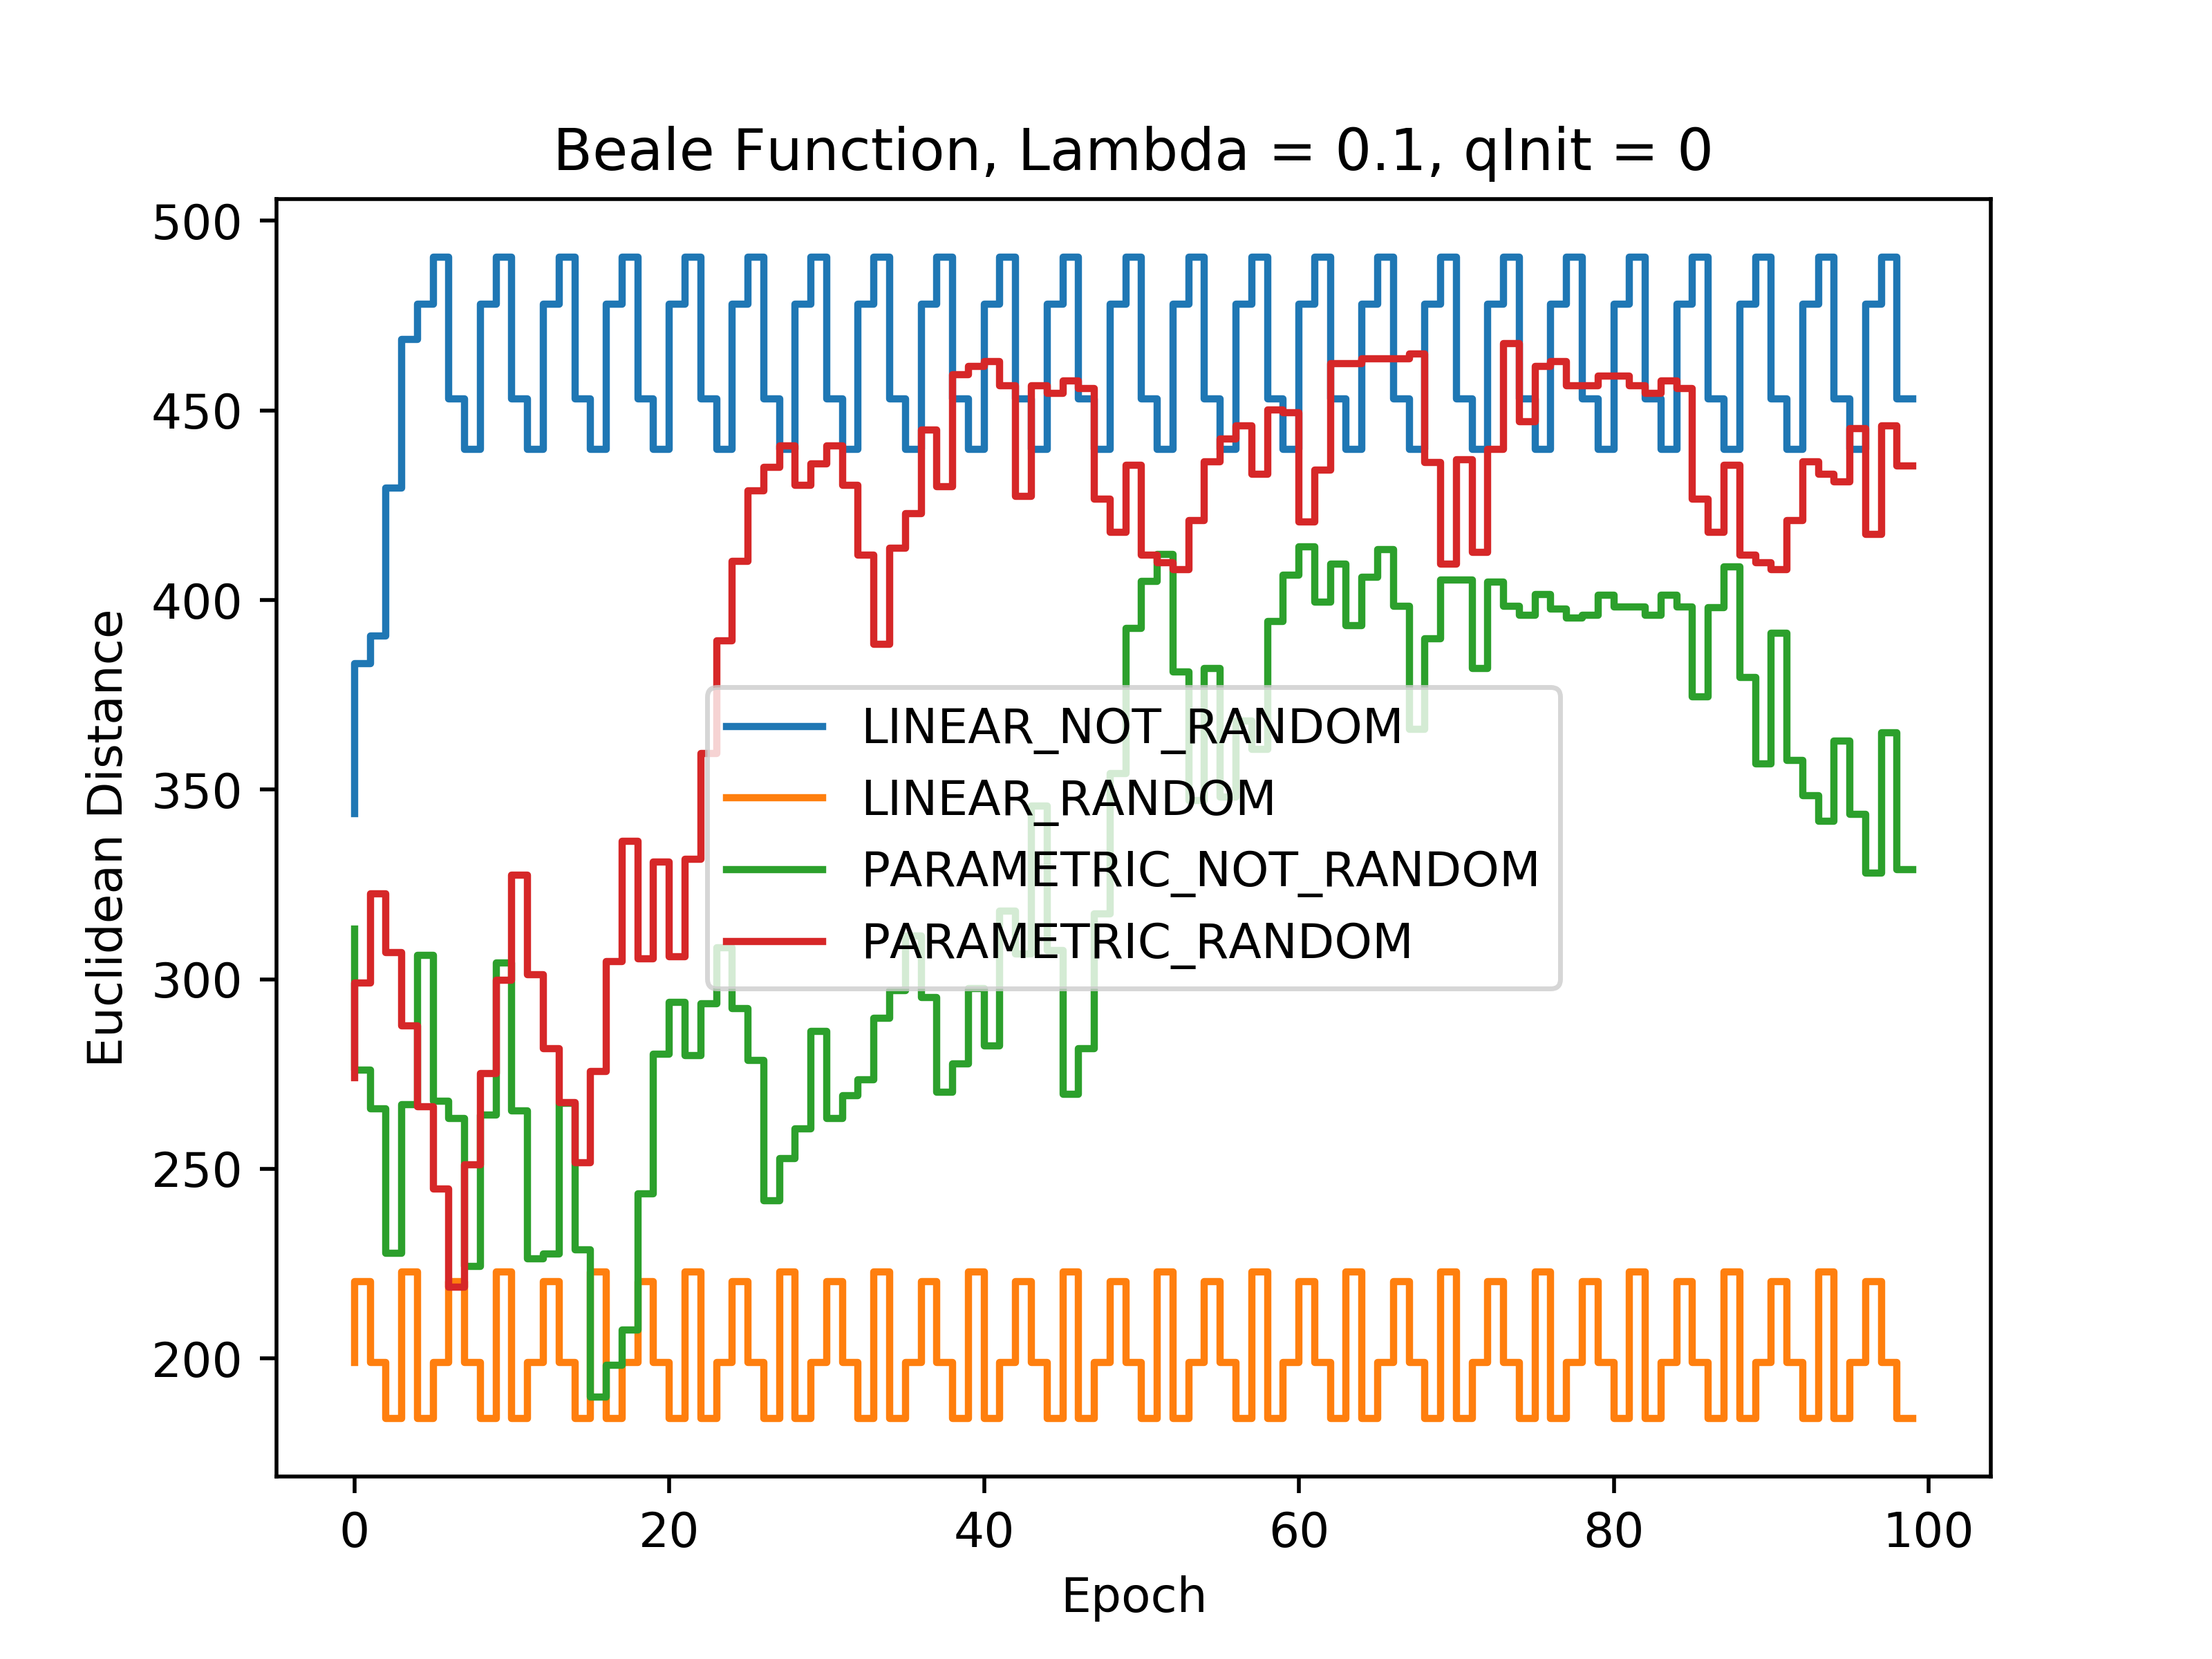
\includegraphics[width=0.4\textwidth]{BealeDifference}
		}
		\subfigure[]{%
			\label{fig:BealeValueFunction}
			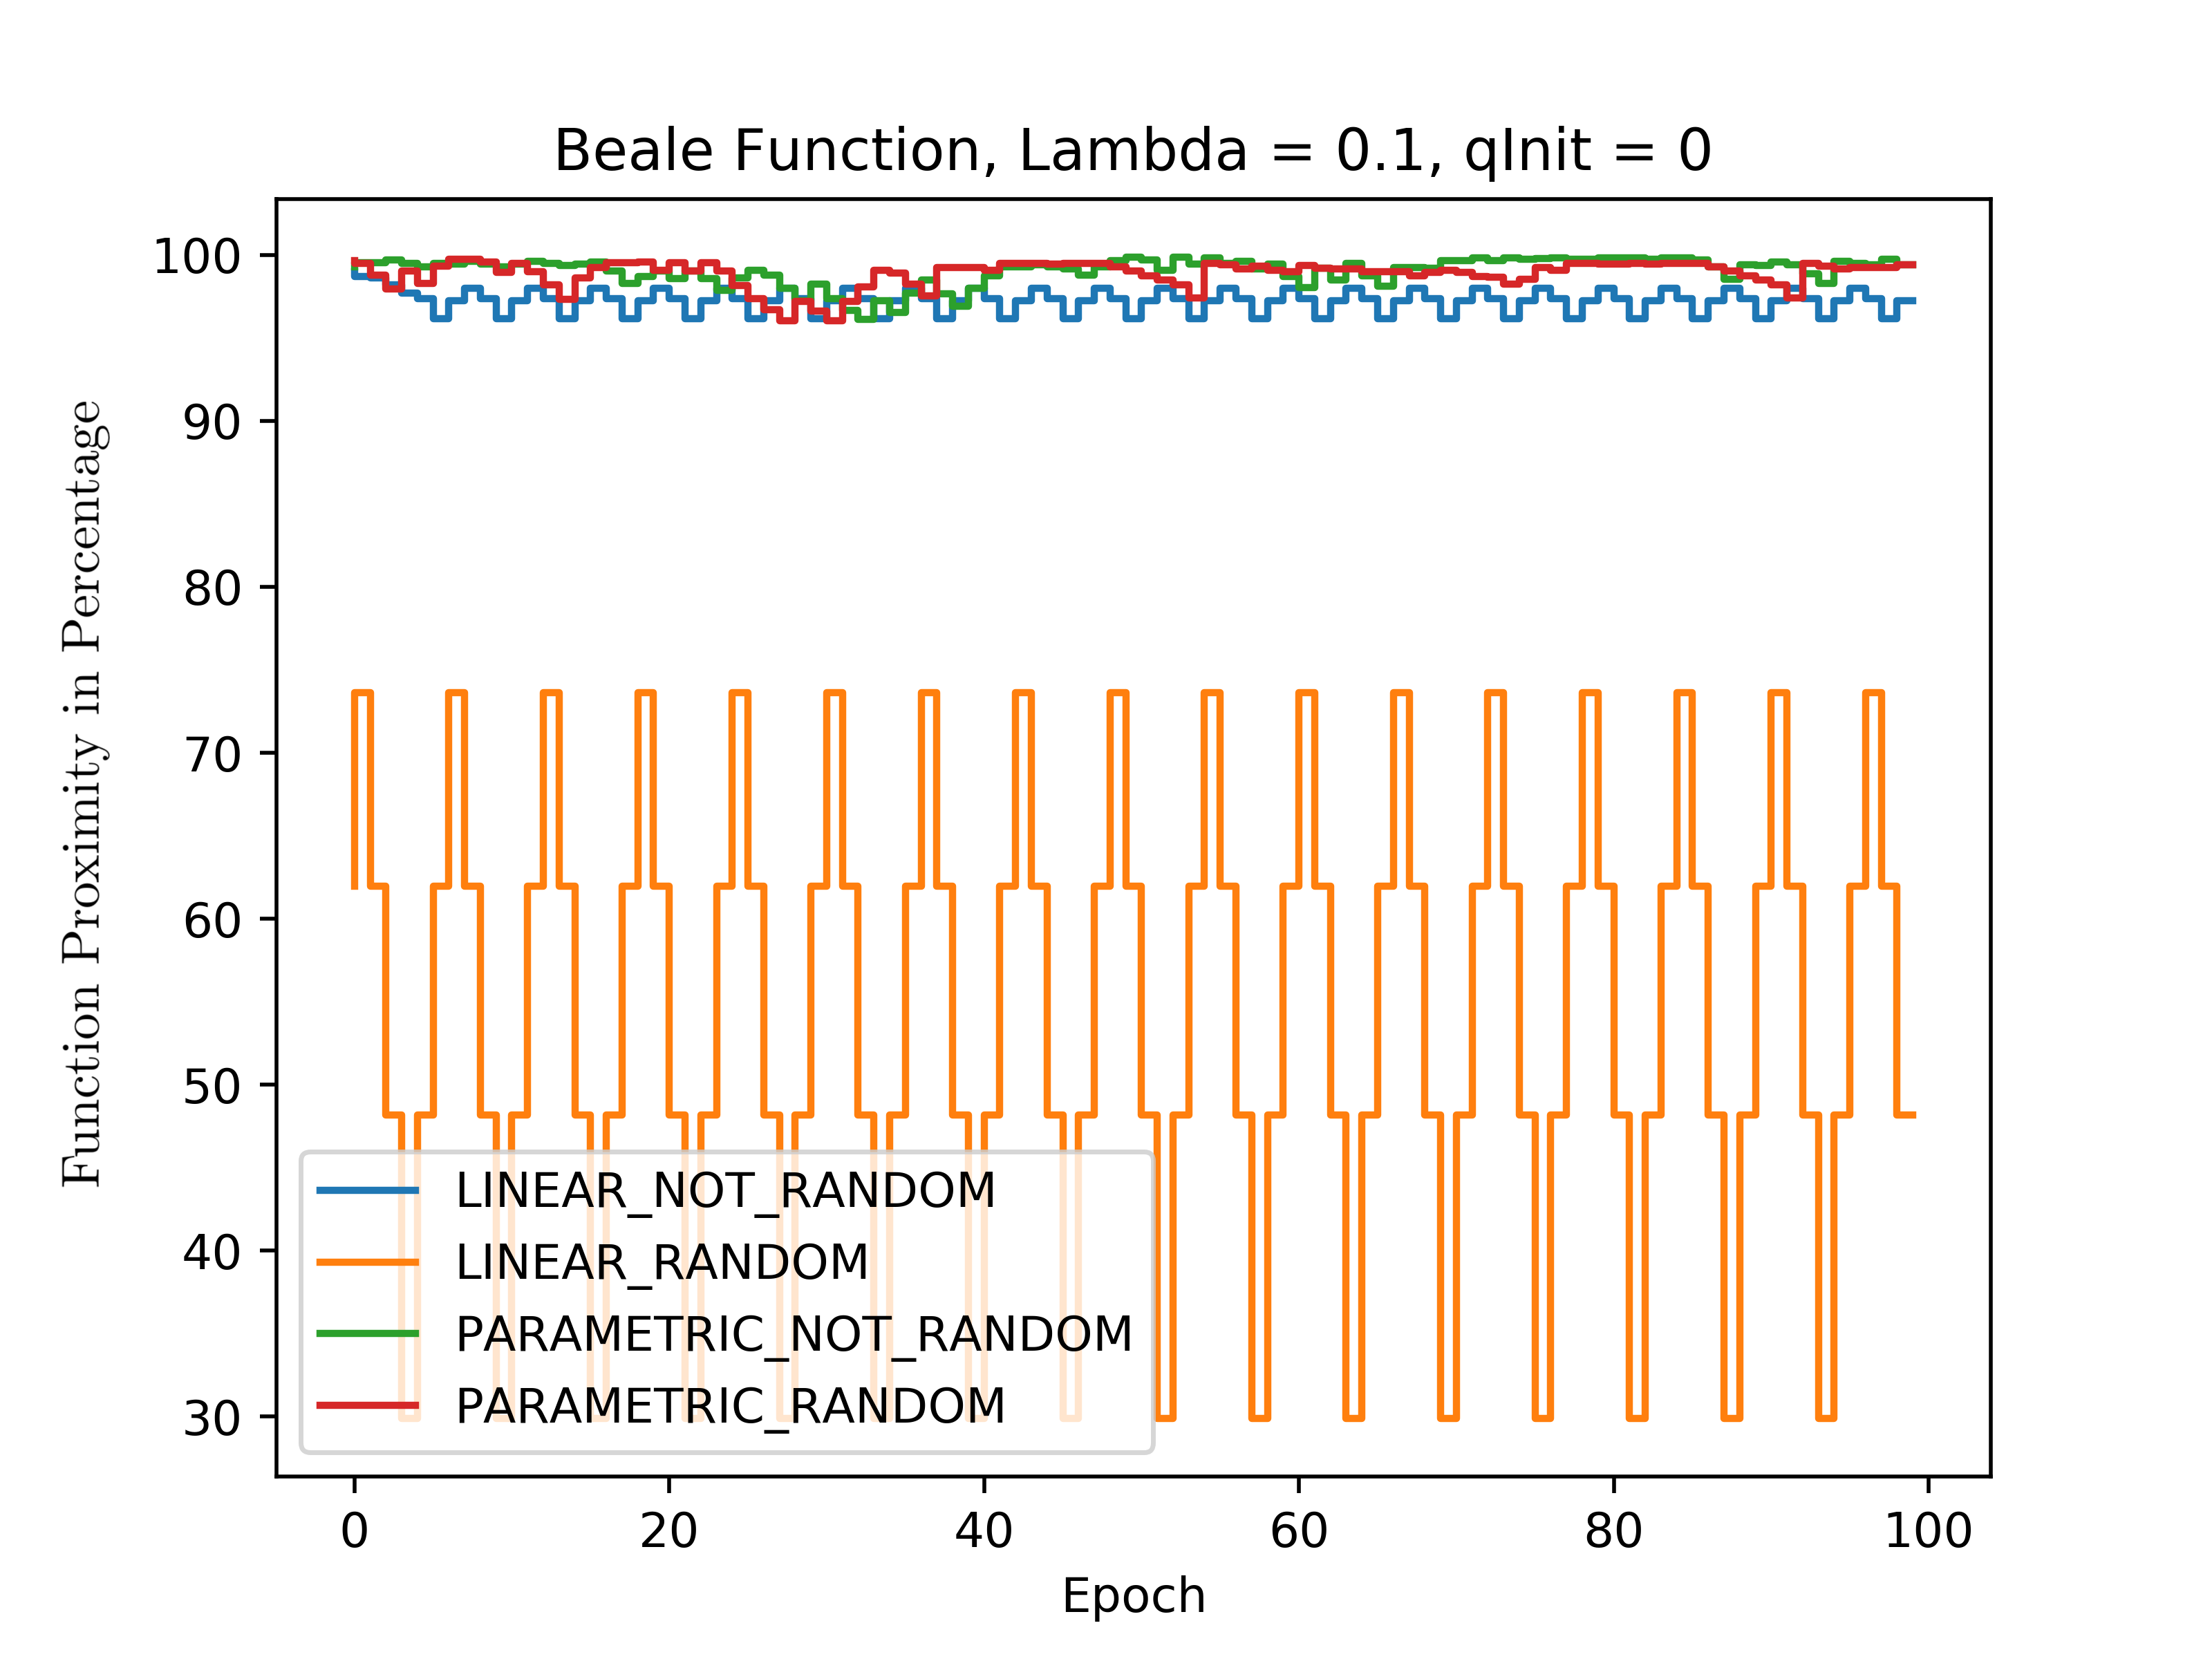
\includegraphics[width=0.4\textwidth]{BealeValueFunction}
		}\\
		\subfigure[]{%
			\label{fig:BealeGap}
			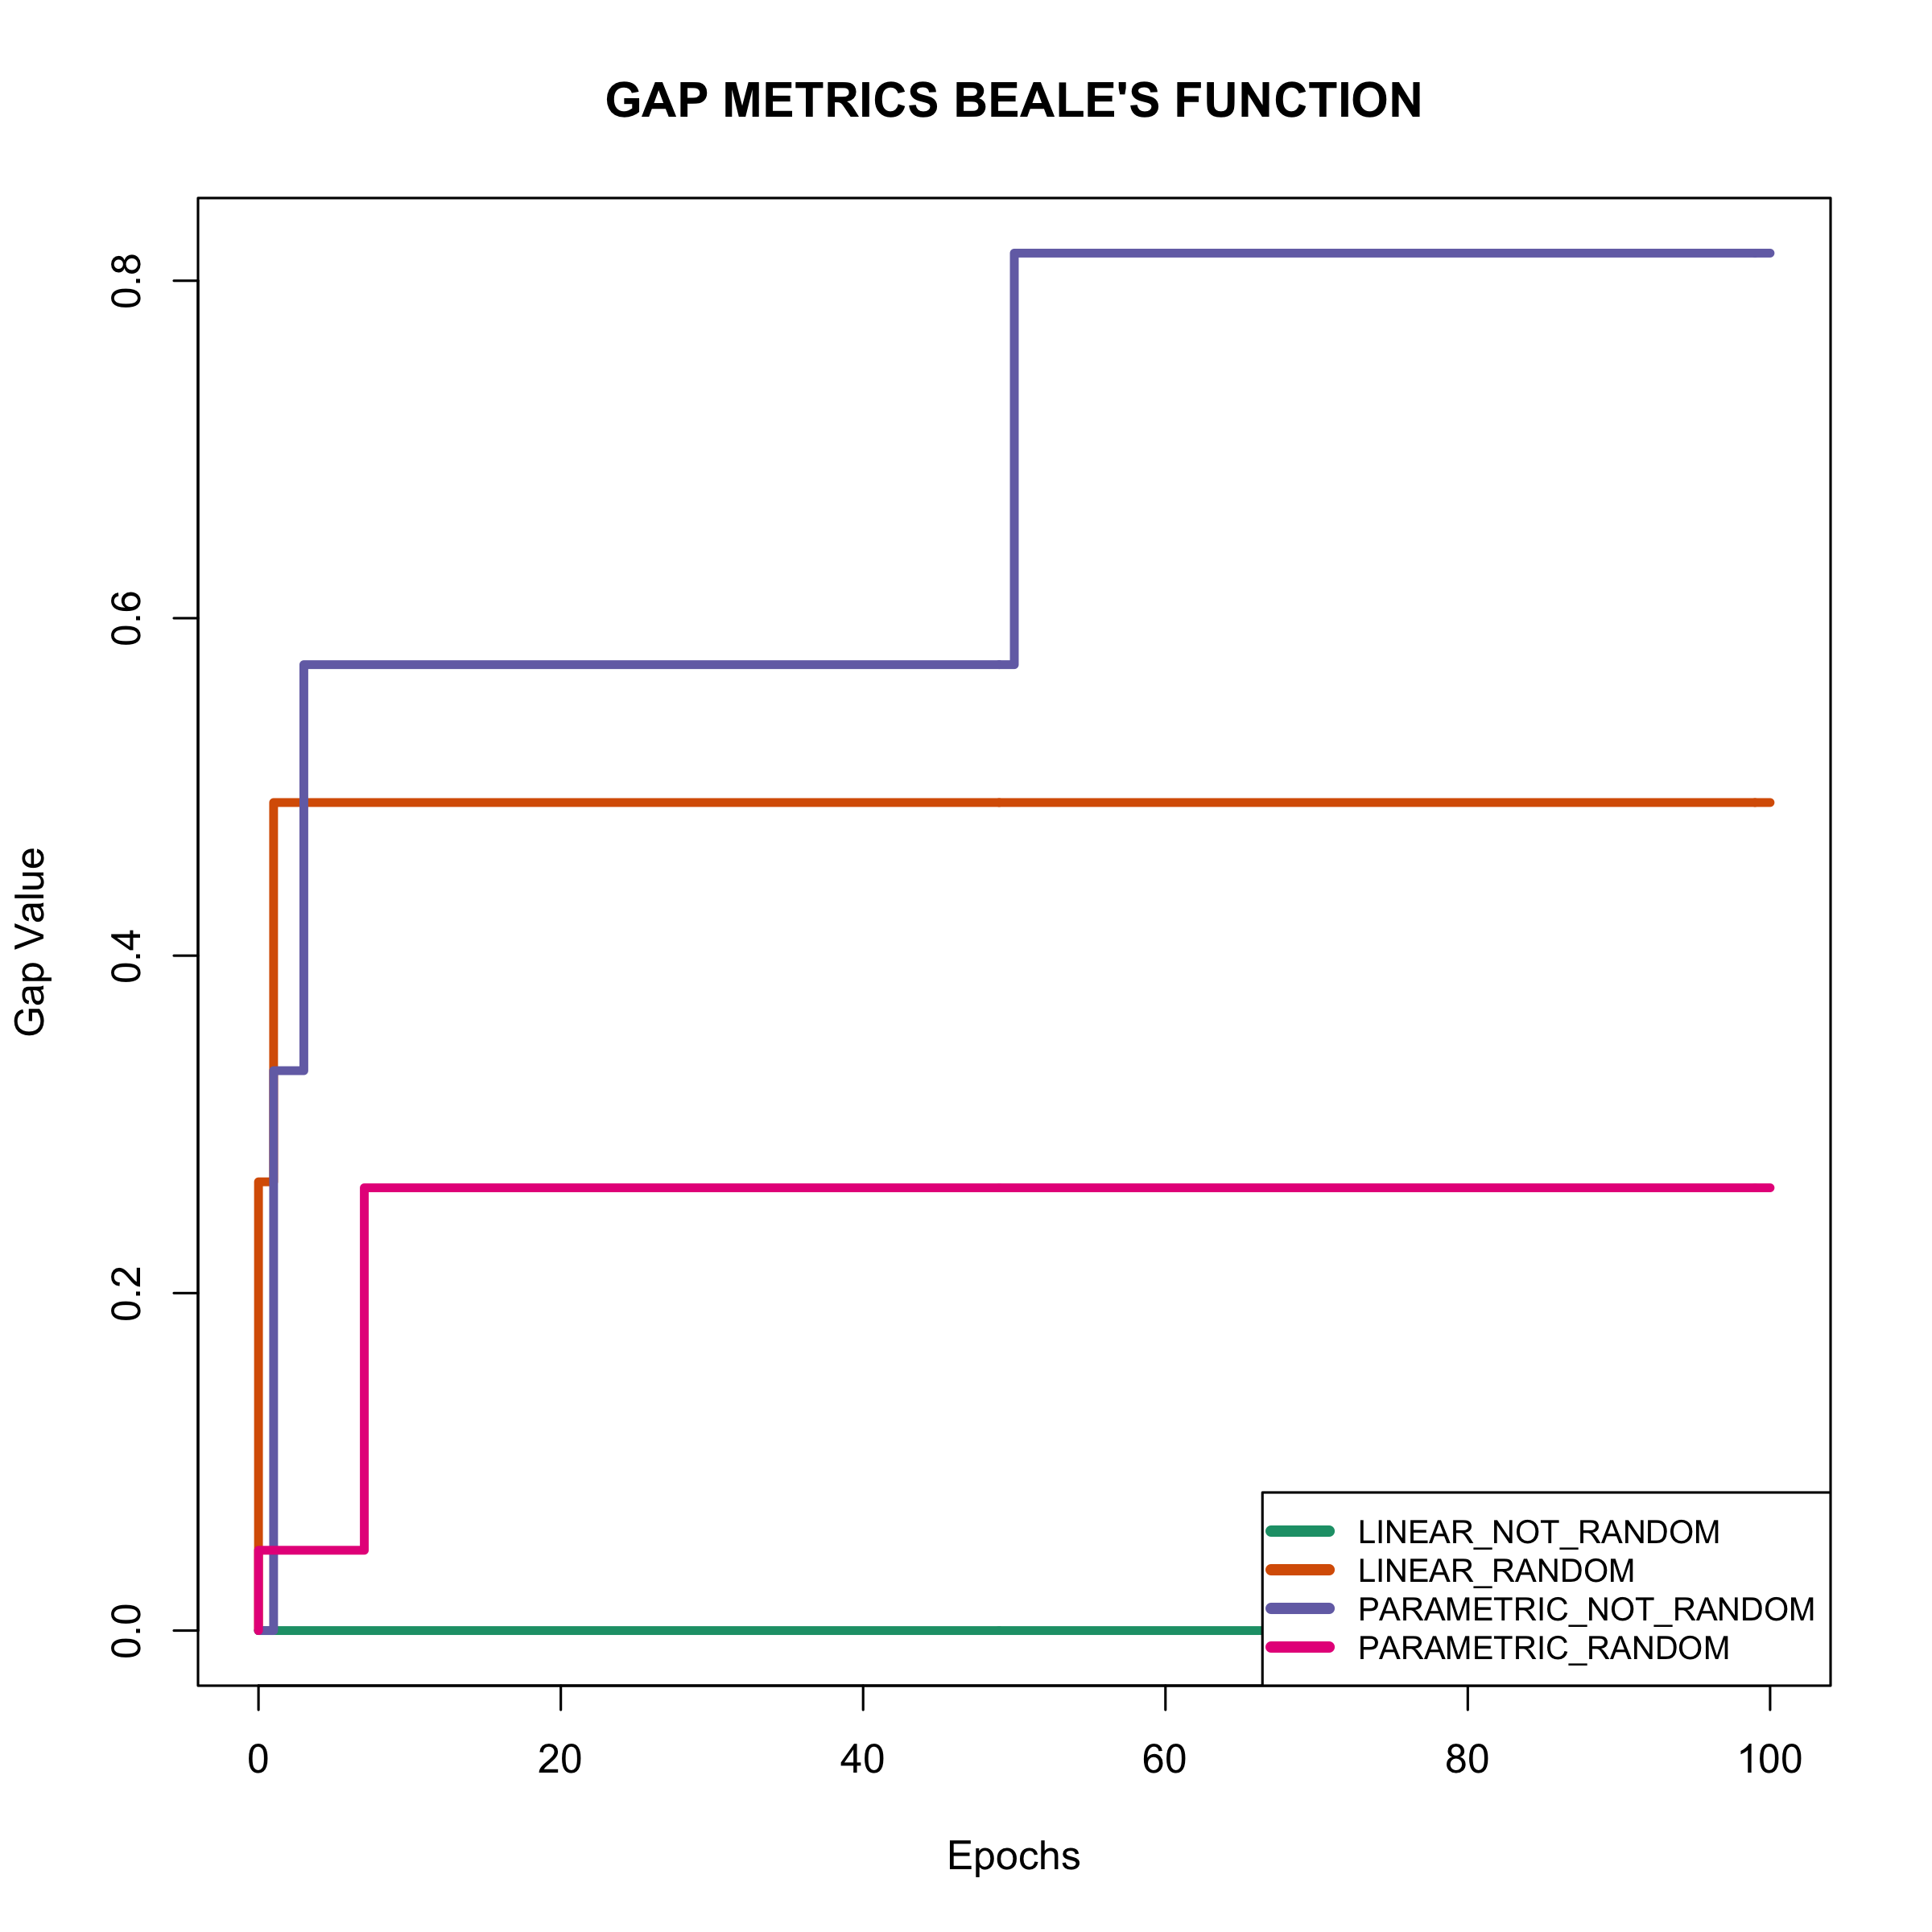
\includegraphics[width=0.4\textwidth]{BealeGap}
		} \\
		
	\end{center}
	\caption{
		Beale Function.
	}
	\label{fig:BealeResults}
\end{figure}

\subsection{Beale Function} Giving an overview to figure \ref{fig:BealeResults} it is possible to see that Beale Function represents the case in which {\tt SARSA($\lambda$)} algorithm' s declinations do worst. 

Plot (a) of figure \ref{fig:BealeResults} graphically represents performances of the four possible declinations of {\tt SARSA($\lambda$)} algorithm obtained considering the \textit{Euclidean distance metric}. Looking at the {\tt linear, not random} declination it is possible to note a growing performance' s worsening until tenth epoch. Starting from epoch ten algorithm's declination starts to stabilize developing a recurrent pattern. Using this declination, the average Euclidean distance from the maximum is $462.4$ pixels.

{\tt Linear, random} declination seems to be the one which performs better. Its average Euclidean distance from the maximum is $201.6$ pixels and its standard deviation is the lowest of the set with a value of $15.4$. This means that it has a relatively good stability. Looking at plot (a) what just said can be easily proved. The current declination starts from a point relatively near to the maximum and never departs from its developing a recurrent pattern.

Looking at {\tt parametric, not random} declination of  {\tt SARSA($\lambda$)} algorithm it is possible to note an high instability. In the very first epochs the distance between the starting point and the maximum slowly decreases, but starting from epoch thirty it starts to messily increase achieving a level near to $350$ pixels. This high instability is reflected also in the high level of standard deviation (table $5.5$).

{\tt Parametric, random} declination combines instability and inaccuracy. It starts from a distance of about $300$ pixels and messily increase its. Its performance is the worst one with an average Euclidean distance of $402.99$ pixels and a standard deviation of $66.6$ (table $5.5$).

Generally speaking it is possible to affirm that those bad performances are the result of an inadequate training space and of a particular function's shape. In addition to this, as already explained, parametric declinations do worst than corresponding ones because of the reduced amount of movement at each epoch. The relatively better performance of {\tt linear, random} declination depends on the possibility to select a starting point closer to the maximum. \\

\begin{table}[h!]
\centering
\resizebox{\linewidth}{!} {
	\begin{tabular}{c| cccccc} 
		\hline \textbf{Beale Function}
		& \textbf{Mean-ED} & \textbf{Standard deviation - ED} \\ 
		\hline Linear not Random
		& $462.4$ & $25.7$\\ 
		\hline Linear Random
		& \cellcolor{red!25}$201.6$ & \cellcolor{red!25}$15.4$\\ 
		\hline Parametric not Random
		& $329.8$ & $62.7$\\ 
		\hline Parametric Random
		& $402.99$ & $66.6$ \\ 
		\hline 
	\end{tabular} 
}
\label{BealeTabEuclidean}
\caption{Euclidean Metric's Performances}
\end{table}

Looking at plot (b) of figure \ref{fig:BealeResults} it is possible to note an inconsistency with what said until now. Only {\tt linear, random} configuration makes an highly swinging performance varying between a percentage of value function' s proximity of about $75\%$ to a percentage of $30\%$. All other declinations make performances around $100\%$ of value function' s proximity. Even looking at table $5.6$ this impression is proved by the high standard deviation of {\tt linear, random} configuration and by the high average of value function' s proximity of all other declinations. These apparently good performances depends on the function' s shape that is very flat. 

\begin{table}[h!]
	\centering
	\resizebox{\linewidth}{!} {
		\begin{tabular}{c| cccccc} 
			\hline \textbf{Beale Function}
			& \textbf{Mean- P} & \textbf{Standard deviation - P} \\ 
			\hline Linear not Random
			& $97.25$ & \cellcolor{green!25}$0.70$\\ 
			\hline Linear Random
			& $54.26$ & $13.89$\\ 
			\hline Parametric not Random
			& \cellcolor{green!25}$99.06$ & $0.81$ \\ 
			\hline Parametric Random
			& $98.88$ & $0.798$ \\ 
			\hline 
		\end{tabular} 
}
	\label{BealeTabProximity}
	\caption{Value Function' s Proximity.} 
\end{table}

Deception can also be revealed by observing plot (c) of figure \ref{fig:BealeResults}. The relatively best performing declination is the {\tt parametric, not random} one which achieves an effectiveness in finding the maximum of about $0.8$ out of $1.0$. It is also proved by table $5.9$. {\tt Parametric, not random} declination achieves point $(-0.77, 1.5599)$ with a value function of $1997.392$ out of $2000$. The worst performing one is the {\tt linear, not random} declination with a constant \textit{gap value} equals to $0$.

\begin{figure}[h!]
	\begin{center}
		\subfigure[]{%
			\label{fig:StyblinskiDifference}
			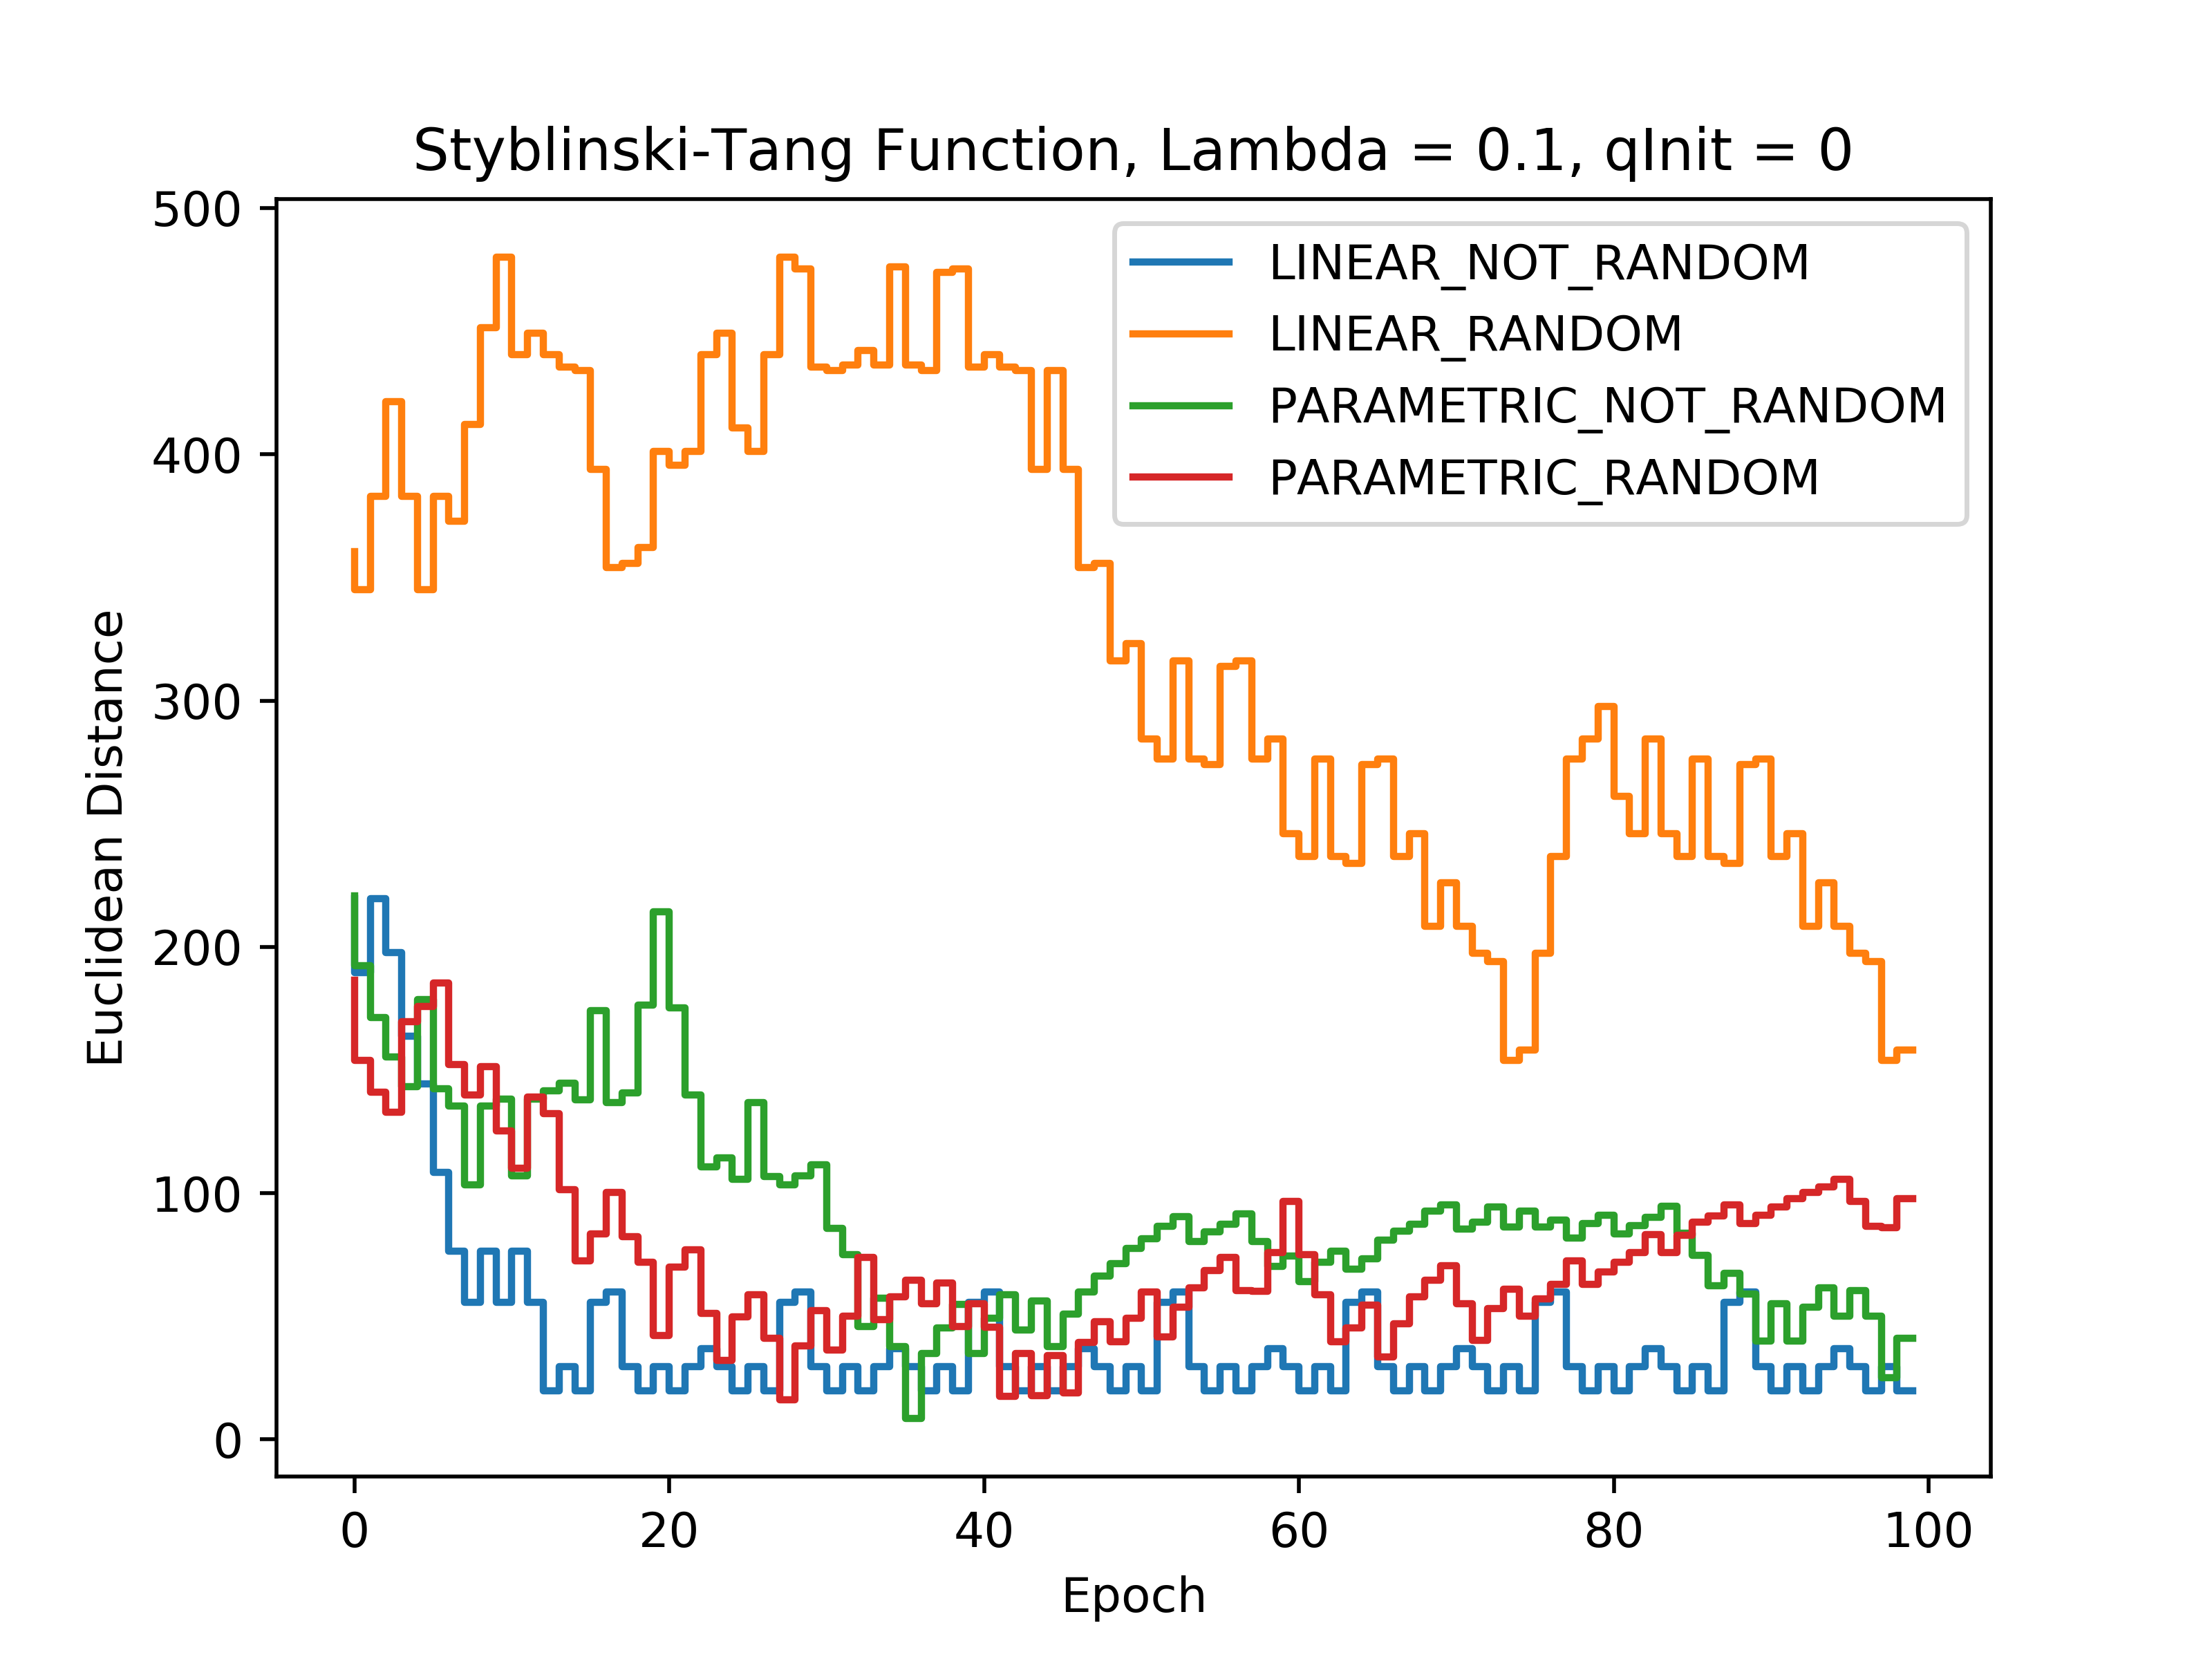
\includegraphics[width=0.4\textwidth]{StyblinskiDifference}
		}
		\subfigure[]{%
			\label{fig:StyblinskiValueFunction}
			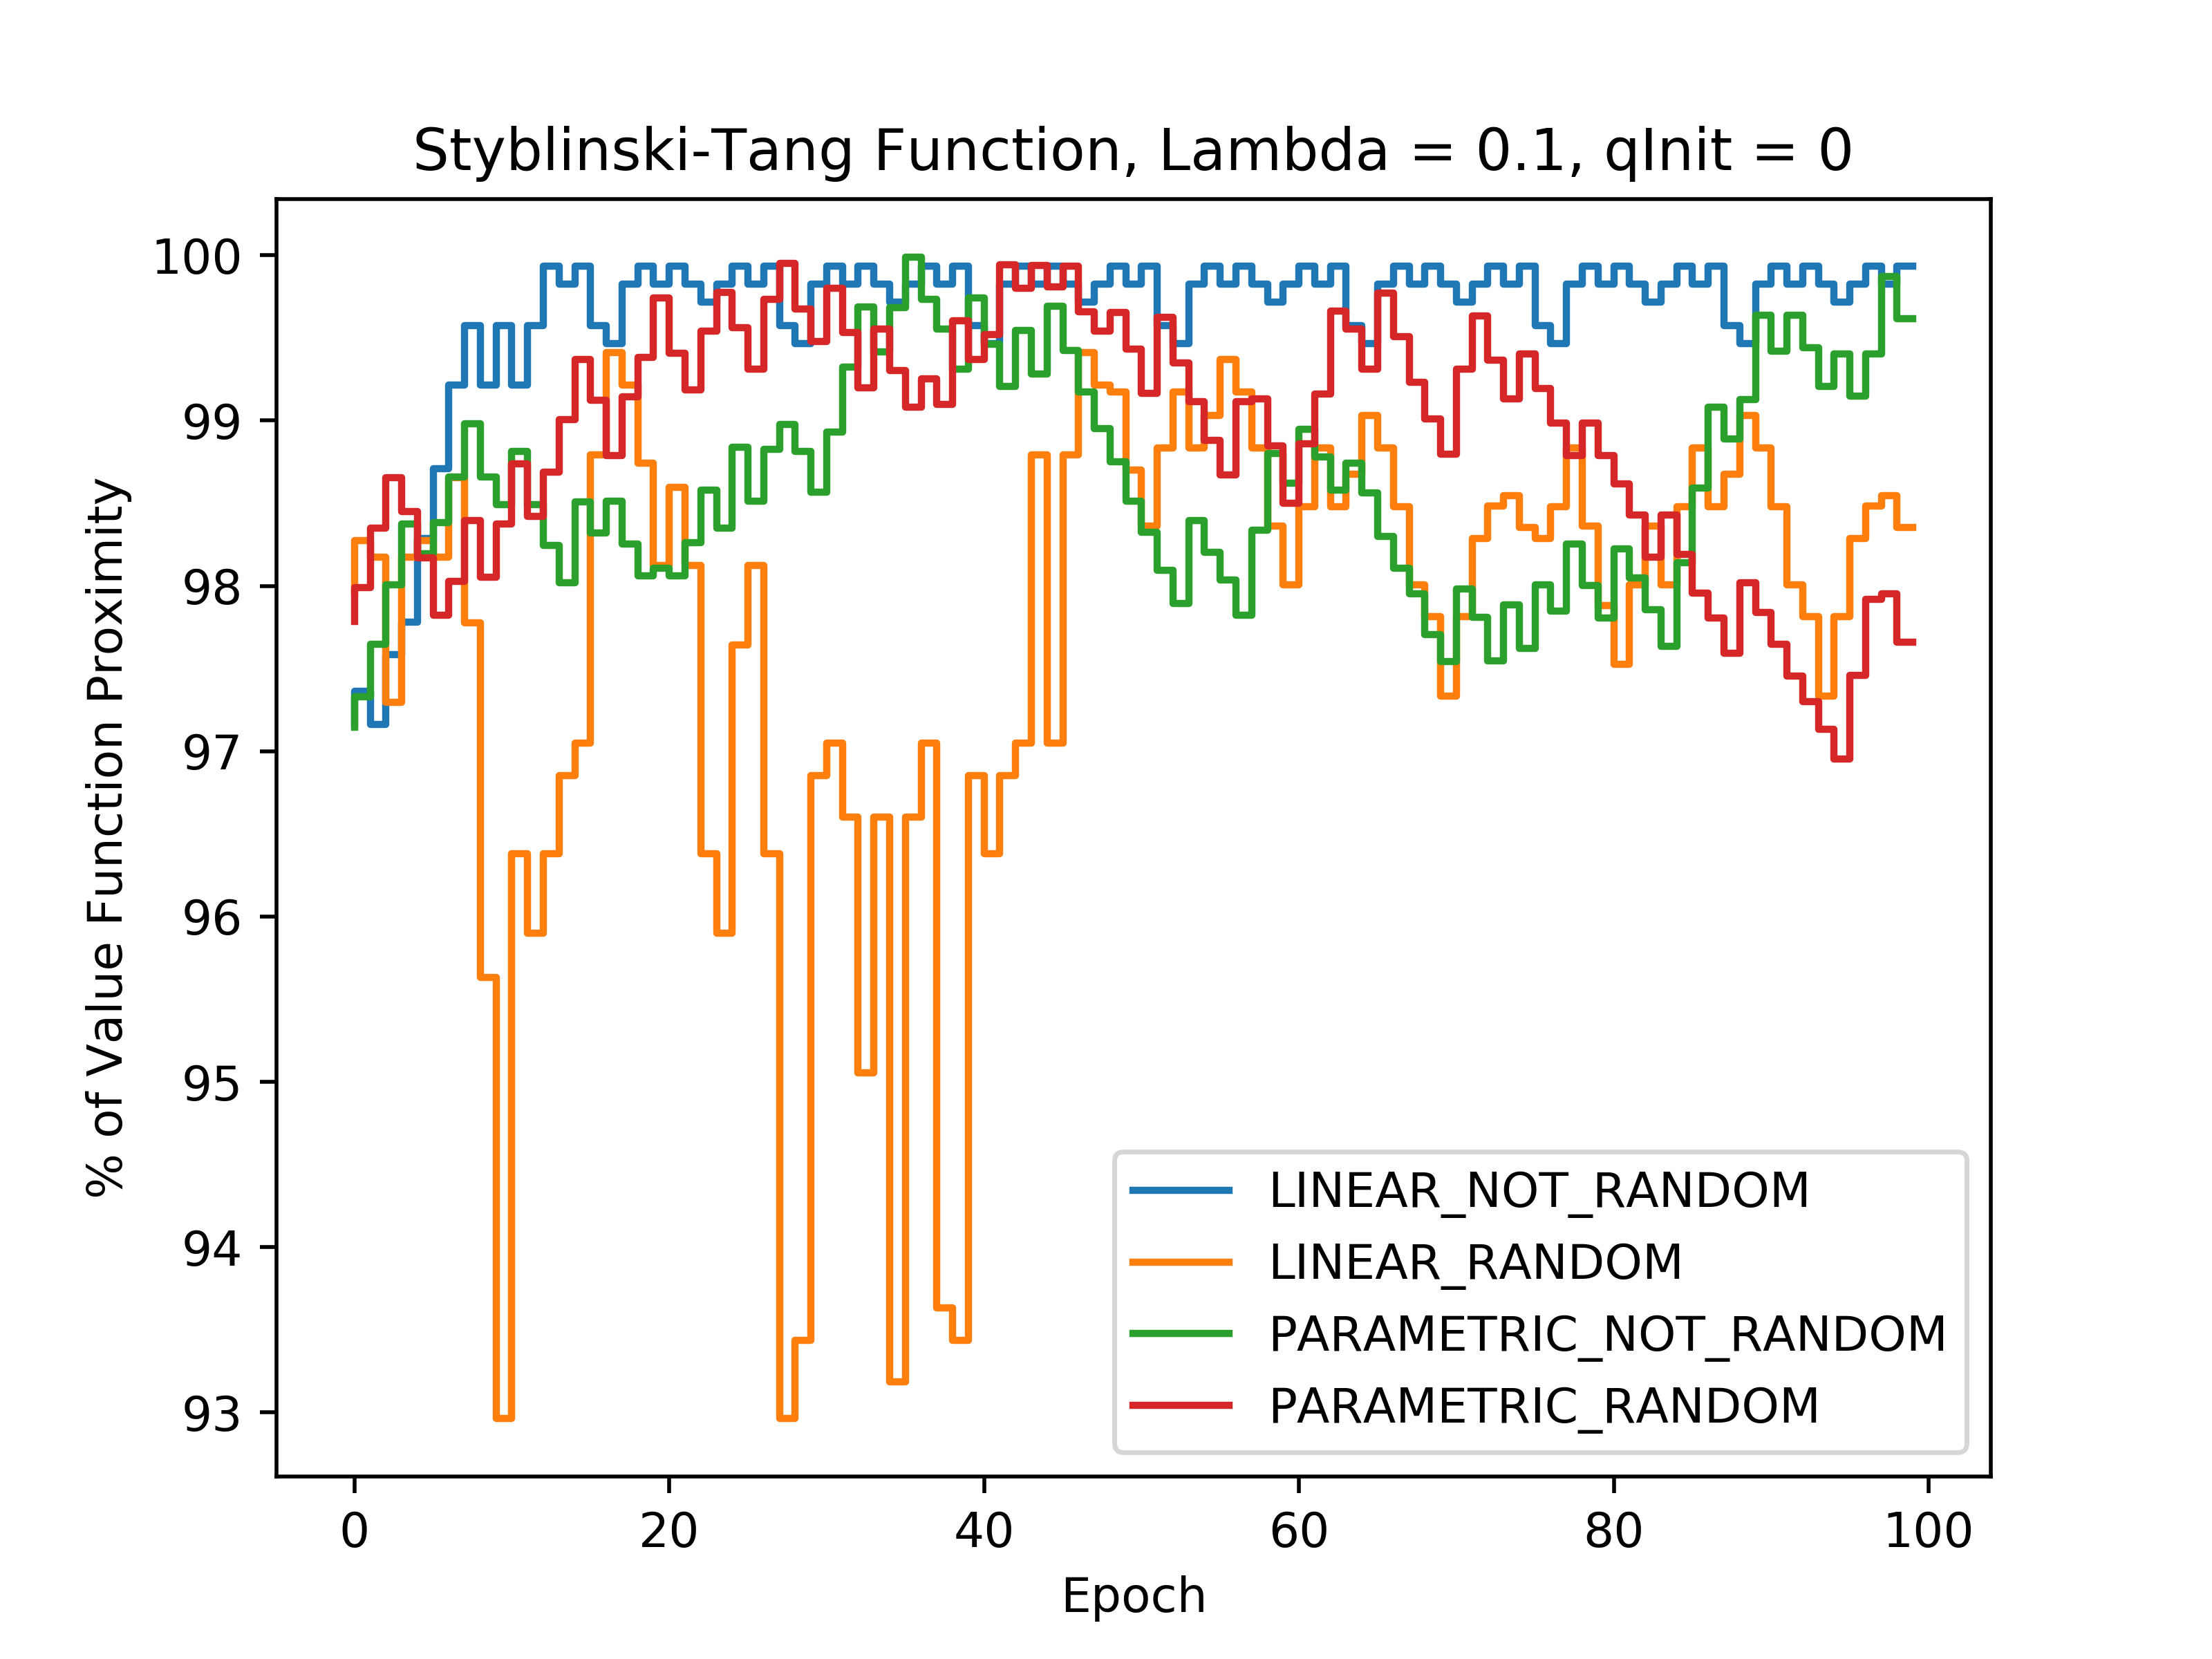
\includegraphics[width=0.4\textwidth]{StyblinskiValueFunction}
		}\\
		\subfigure[]{%
			\label{fig:StyblinskiGap}
			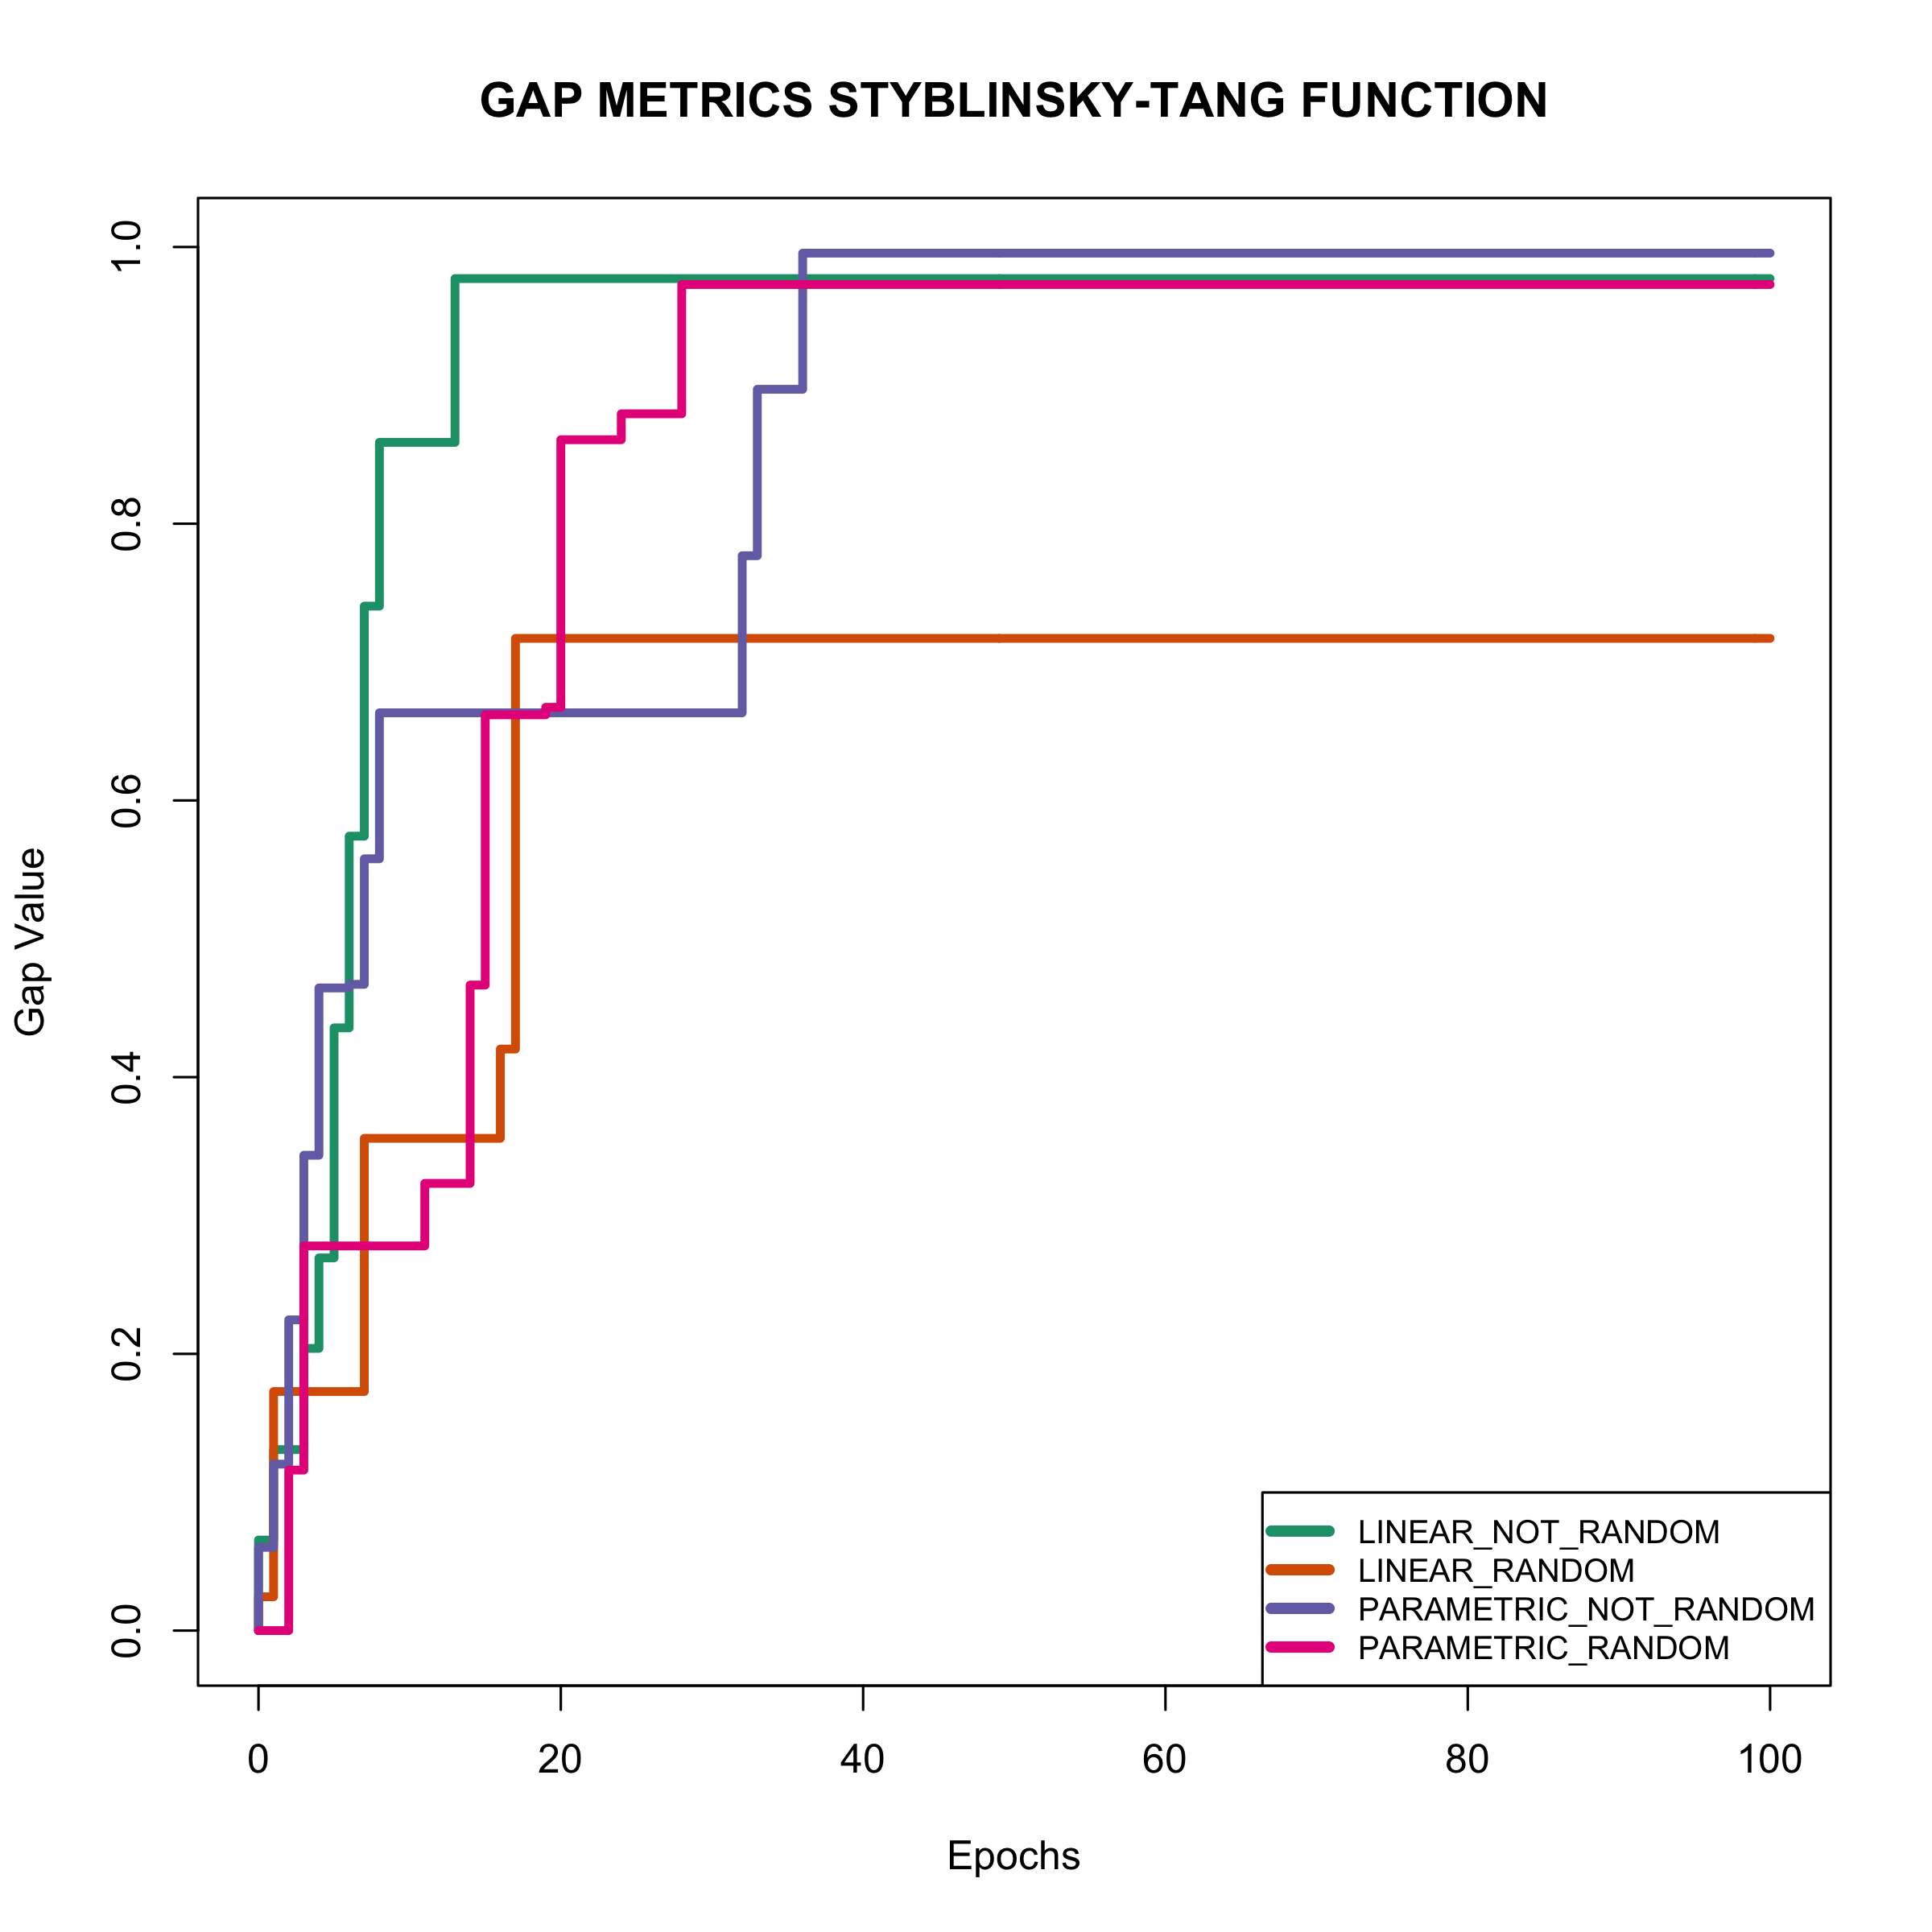
\includegraphics[width=0.4\textwidth]{StyblinskiGap}
		} \\
		
	\end{center}
	\caption{
		Styblinski Function.
	}
	\label{fig:StyblinskiResults}
\end{figure}

\subsection{Styblinski-Tang Revised Function} Plot (a) of figure \ref{fig:StyblinskiResults} graphically represents performances of the four possible declinations of {\tt SARSA($\lambda$)} algorithm obtained considering the \textit{Euclidean distance metric}. 

Looking at the {\tt linear, not random} declination's performance, the Euclidean difference between the agent's position and the global maximum is about $200$ pixels. Staring from the twentieth epoch it starts to stabilize around an Euclidean distance level from the maximum of about $40$ pixels. Note that in less than twenty epochs the Euclidean distance from the maximum is about the $20\%$ of the starting one. The current declination also reveals a great stability. With an average Euclidean distance of $43.63$ pixels and a standard deviation of $41.05$, the {\tt linear, not random} declination is the best of the set (table $5.7$).

A decisively worse performance is given by the {\tt linear, random} declination. It starts with an Euclidean distance from the maximum of about $360$ pixels and messily decreases until achieving a level of $180$ pixels. The noise just described is also proved by the highest average Euclidean distance and by the highest standard deviation of the set (table $5.7$).

Last two, parametric declinations give for the first time the possibility to really see behaviour of parametric declination. Starting from about the fiftieth epoch, {\tt parametric, not random} movement starts to imperceptibly increase. This lower amount of movement compared to the non parametric movements depends on the definition of the parametric movement itself. The same behaviour can be seen in {\tt parametric, random} declination starting from epoch $75$. This declination performs better then the {\tt parametric, not random} one in the first epochs but it performs worse in the last ones. With an average Euclidean distance from the maximum of $75.26$ pixels, and with an average standard deviation of $37.34$, the {\tt parametric, random} declinations is generally better than the {\tt parametric, not random} one.

\begin{table}[h!]
	\centering
	\resizebox{\linewidth}{!} {
		\begin{tabular}{c| cccccc} 
			\hline \textbf{Styblinski-Tang Function}
			& \textbf{Mean-ED} & \textbf{Standard deviation - ED} \\ 
			\hline Linear not Random
			& \cellcolor{red!25}$43.63$ & \cellcolor{red!25}$41.05$\\ 
			\hline Linear Random
			& $330.16$ & $95.39$ \\ 
			\hline Parametric not Random
			& $91.79$ & $42.24$\\ 
			\hline Parametric Random
			& $75.26$ & $37.34$\\ 
			\hline 
		\end{tabular} 
	}
	\label{StyblinskiTabEuclidean}
	\caption{Euclidean Metric's Performances}
\end{table}

The performance just described is also proved by the percentage of value function' s proximity to the maximum. With an average mean of $99.63\%$ of precision, and a standard deviation of $0.57$, the {\tt linear, not random} declination is the best of the set. General good performances are also made by all other declinations except for the {\tt linear, random} one. Looking at plot (b) of figure \ref{fig:StyblinskiResults} it is possible to note an high instability of this last declination especially until epoch fifty. It than starts to stabilize varying between a proximity level of $97\%$ and $99\%$.

\begin{table}[h!]
	\centering
	\resizebox{\linewidth}{!} {
		\begin{tabular}{c| cccccc} 
			\hline \textbf{Styblinski-Tang Function}
			& \textbf{Mean- P} & \textbf{Standard deviation - P}\\ 
			\hline Linear not Random
			& \cellcolor{green!25}$99.63$ & \cellcolor{green!25}$0.57$ \\ 
			\hline Linear Random
			& $97.73$ & $1.46$ \\ 
			\hline Parametric not Random
			& $98.61$ & $0.66$\\ 
			\hline Parametric Random
			& $98.90$ & $0.74$\\ 
			\hline 
		\end{tabular} 
	}
	\label{StyblinskiTabProximity}
	\caption{Value Function' s Proximity.} 
\end{table}

Looking at the third plot it is possible to note that the best performance is the one of the {\tt parametric, not random} declination. This result obviously depends on the fact that around the thirty-ninth epoch it reaches the maximum for then decisively distance itself from it. This behaviour is again due to the absence of an adequate training space. This lack prevents the agent from developing an optimal policy.

\begin{sidewaystable} 
	\centering
	\label{table:BestSoundings}
	\caption{Best Soundings}
	\begin{tabular}
		{l l l l l} \hline Name & Linear Not Random & Linear Random & Parametric Not Random & Parametric Random \\
		\hline Himmelblau & \vtop{\hbox{\strut $2486.938$}\hbox{\strut $(2.67, 1.34)$}\hbox{\strut}\hbox{\strut}} &\cellcolor{blue!25} \vtop{\hbox{\strut $2498.457$}\hbox{\strut $(3.67, -1.57)$}\hbox{\strut}\hbox{\strut}} & \vtop{\hbox{\strut $2485.972$}\hbox{\strut $(-2.1, 3.30)$}\hbox{\strut}\hbox{\strut}} & \vtop{\hbox{\strut $2492.11$}\hbox{\strut $(-2.283, 3.234)$}\hbox{\strut}\hbox{\strut}} \\
		Sphere & \vtop{\hbox{\strut $3484.44$}\hbox{\strut $(-8.8, -0.67)$}\hbox{\strut}\hbox{\strut}} & \vtop{\hbox{\strut $3537.986$}\hbox{\strut $(-3.24, 3.40)$}\hbox{\strut}\hbox{\strut}} &\cellcolor{blue!25} \vtop{\hbox{\strut $3557.722$}\hbox{\strut $(-1.034, -1.099)$}\hbox{\strut}\hbox{\strut}} & \vtop{\hbox{\strut $3553.626$}\hbox{\strut $(1.69, 1.88)$}\hbox{\strut}\hbox{\strut}} \\
		Beale & \vtop{\hbox{\strut $1985.797$}\hbox{\strut $(0, 0)$}\hbox{\strut}\hbox{\strut}} & \vtop{\hbox{\strut $1472.184$}\hbox{\strut $(1.69, 2.269)$}\hbox{\strut}\hbox{\strut}} &\cellcolor{blue!25} \vtop{\hbox{\strut $1997.392$}\hbox{\strut $(-0.77, 1.559)$}\hbox{\strut}\hbox{\strut}} & \vtop{\hbox{\strut $1994.983$}\hbox{\strut $(1.309, -0.89)$}\hbox{\strut}\hbox{\strut}} \\
		Styblinski-Tang & \vtop{\hbox{\strut $5153.086$}\hbox{\strut $(-2.67, -2.67)$}\hbox{\strut}\hbox{\strut}} & \vtop{\hbox{\strut $5126.192$}\hbox{\strut $(3, -2.97)$}\hbox{\strut}\hbox{\strut}} &\cellcolor{blue!25} \vtop{\hbox{\strut $5155.97$}\hbox{\strut $(-2.77, -2.95)$}\hbox{\strut}\hbox{\strut}} & \vtop{\hbox{\strut $5154.053$}\hbox{\strut $(-3.17, -2.99)$}\hbox{\strut}\hbox{\strut}} \\
		\hline
	\end{tabular}
\end{sidewaystable}